\documentclass[11pt,a4paper,footexclude,headsepline,footsepline,BCOR12mm,DIV13]{scrbook}
\usepackage[utf8]{inputenc}
\usepackage[english,german]{babel}
\usepackage{amsmath}
\usepackage{amsfonts}
\usepackage{amssymb}
\usepackage{graphicx}
\usepackage{styles/tumlogo}
\graphicspath{{images/}}
\usepackage{algorithm,algorithmic}
\usepackage{url}
\usepackage{hyperref}
\usepackage{todo}

\usepackage{bm} % Use \bm{\theta} 

\usepackage{mathtools}	% for small minus
\newcommand*{\matminus}{%
  \leavevmode
  \hphantom{0}%
  \llap{%
    \settowidth{\dimen0 }{$0$}%
    \resizebox{1.1\dimen0 }{\height}{$-$}%
  }%
}

\newcommand*{\matplus}{	% for small plus
	\text{+}
}

% remove indent after newline
\setlength\parindent{0pt}

% for rotated matrix
\usepackage{mathtools}
\usepackage{rotating}

% for pdf_tex
\usepackage{import}
\usepackage{xcolor}

\author{Anna Baumeister}
\title{Path Planning for an Ophthalmic Surgical Robot using V-REP}
\begin{document}

\thispagestyle{empty}

\vspace{4cm}
\begin{center}
  \oTUM{4cm}

  \vspace{5mm}
  \huge FAKULT{\"A}T F{\"U}R INFORMATIK\\
  \vspace{0.5cm}
  \large DER TECHNISCHEN UNIVERSIT{\"A}T M{\"U}NCHEN\\
  \vspace{1mm}

\end{center}


\vspace{15mm}
\begin{center}

  {\Large Bachelor's Thesis in Engineering Science}

  \vspace{20mm}

  {\huge\textbf{The Needle Detection and Reconstruction Based on OCT image with GPU Acceleration}}\\%[3ex]


  \vspace{15mm}


  {\LARGE  Anh Tuan Pham}


  \vspace{5mm}
  


  \begin{figure}[h!]
    \centering
    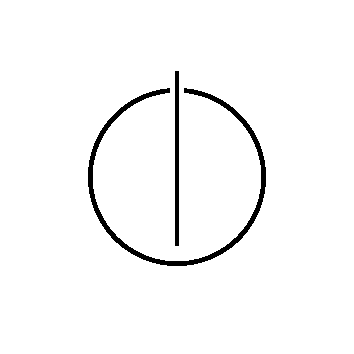
\includegraphics[width=4cm]{styles/informat.png}
  \end{figure}


\end{center}
\cleardoublepage
% The titlepage for the CAMP report document.
% Included by MAIN.TEX


% --------------------------------------------------
% The title page
% --------------------------------------------------

% correct BCOR - undo at the end !!!
% \def\bcorcor{0.15cm}
% \addtolength{\hoffset}{\bcorcor}

\thispagestyle{empty}

\vspace{7mm}
\begin{center}
  \oTUM{4cm}

  \vspace{5mm}
  \huge FAKULT{\"A}T F{\"U}R INFORMATIK\\
  \vspace{0.5cm}
  \large DER TECHNISCHEN UNIVERSIT{\"A}T M{\"U}NCHEN
\end{center}
\vspace{7mm}
\begin{center}

  {\Large Bachelor's Thesis in Engineering Science}

  \vspace{7mm}

  {\LARGE \textbf{Path Planning for an Ophthalmic Surgical Robot using V-REP}}\\

  \vspace{5mm}

  {\LARGE  	\textbf{Pfadplanung für einen Assistenzroboter in der Augenchirurgie mit V-REP}}\\

  \vspace{10mm}

  % \hfill
  \begin{tabular}{ll}
    \Large Author:     & \Large Anna Baumeister \\[2mm]
    \Large Supervisor:    & \Large Prof. Dr.-Ing. habil. Alois Knoll\\[2mm]
    \Large Advisor:	& \Large Mingchuan Zhou, M.Sc.\\[2mm]
    \Large Date:       & \Large \today
  \end{tabular}

  \vspace{5mm}

   \begin{figure}[h!]
     \centering
     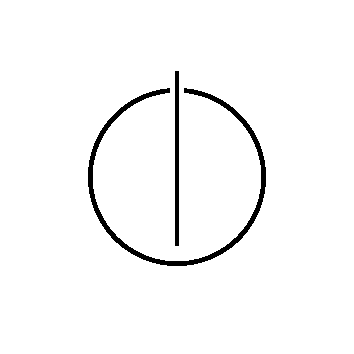
\includegraphics[width=4cm]{styles/informat.png}
   \end{figure}

  \vspace{10mm}

\end{center}

% undo BCOR correction
% \addtolength{\hoffset}{\bcorcor}

\cleardoublepage


%\thispagestyle{empty}

\vspace*{0.7\textheight}
\selectlanguage{english}
\noindent I assure the single handed composition of this bachelors's thesis only supported by declared resources.
\selectlanguage{german}

\vspace{7mm}

\noindent Ich versichere, dass ich diese Bachelorarbeit selbst\"andig verfasst und nur die angegebenen Quellen und Hilfsmittel verwendet habe.
\selectlanguage{english}

\vspace{12mm}

\selectlanguage{english}
\noindent Munich, September 14, 2017

\vspace{7mm}

\selectlanguage{german}
\noindent M\"unchen, den 14. September 2017 \hspace{3cm}  Anna Baumeister
\newpage
\selectlanguage{english}
\vspace{1cm}
I would like to thank my advisors Mingchuan Zhou and Professor Alois Knoll for their impossible patience and  aspiration. And to Mai Linh for proofreading this thesis with my horrible grammar. And to my mother, for supporting everything i do.

\cleardoublepage

\vspace*{2cm}
\begin{center}
{\Large \textbf{Abstract}}
\end{center}
\vspace{1cm}
In the recent years the medical world has witnessed a growing popularity of robot aided surgeries in various operations. This technical development has shown very promising results: Robot-aided operations are being done with better precision, miniaturization, decreased blood loss, less pain, and quicker healing time (?). 

Up to pace with the development, a robot with focus on eye surgeries is being developed by the Department of Robotics, TU Munich. The robot is designed to provide assistance in drug injections into the eye vessels, which is currently carried out by human surgeons. The complex nature of the human anatomy makes a needle penetration a challenging procedure. It requires a very high level of precision, whereas a small mistake could cause very costly damages to the eyes. Humans are not immune to errors, a tremor in the hands or a slightly suboptimal needle pose could not be totally prevented, and therefore a robot is particularly advantageous in this scenario.

One important part of robot development is to calculate the position and rotation of the needle at real-time, as accurately as possible. This task could demand a lot of effort. Ramona Schneider had successfully developed a robust algorithm in her master thesis to execute the calculation. The key element of this approach is to use Optical Coherence Tomography (OCT) images to compute the direction, x- and y-rotation of the needle. The remaining parameters, z-rotation and shift, are computed by defining intervals and combining values inside them. The combination with the most corresponding points is used for the transformation of the CAD model.

While the thesis showed great results, the execution still requires a lot of CPU resources and requires too much time for a real time system. Depending on the CPU used, the execution could take from 2 up to 3 seconds for each frame. The goal of this thesis is to find another approach to optimize the execution of the same algorithm, to reach a fastest execution time as possible.

Based on the nature of this algorithm, which is executing a lot of matrix calculations, a Graphic Processing Unit with far more superior number of threads available is more suitable for the task. In this thesis all of the calculations are executed parallelly on a GPU device with the help of OpenCL. Therefore the code was re-implemented in adjustment and optimization for GPU programming practice. The result is quite encouraging: for the same input and number of combinations, the optimized approach showed a 10x faster execution time, which is 20-30 milliseconds a frame without the best equipments. 



\tableofcontents{}


\chapter{Introduction}

\section{Objectives of this Thesis}
Subject of this thesis is the ophthalmic surgical robot developed in the iRAM!S project \cite{iramis}. When performing minimally invasive surgery, an important task is to prevent lateral movement of the tool at the point of incision to minimize strain on the surrounding tissue. In the iRAM!S project, this is achieved by defining a point on the needle as a Remote Center of Motion (RCM) and algorithmically forcing its velocity to zero. This thesis focuses on the following topics regarding the implementation of a virtual RCM:
\begin{itemize}
	\item Recalculation and verification of the Jacobian matrix for the surgical robot, both for unconstrained and constrained movement. For this purpose a model of the robot is implemented in the V-REP simulation environment.
	\item In the simulation environment, performing an injection at multiple sites of the inner eye surface and measuring the deviation of the RCM point  from its optimal position.
	\item Finding a set of control parameters that ensures that the needle pose quickly converges to any target pose within the workspace of the robot while maintaining the RCM position. 
	\item Comparing the performance of the Jacobian pseudoinverse method to V-REPs built-in inverse kinematics solver, which employs a Dampened Least Squares method, to get an estimate for the possible accuracy.
\end{itemize} 

\section{Robotic Assisted Minimally Invasive Surgery}

In recent years, robotic assistance has gained increasing acceptance in clinical practice, mainly due to improvements in precision, reliability and ergonomics. Most of these systems, referred to as \textit{surgical assistants}, are designed to enhance the ability of a surgeon to perform a certain procedure with additional tools. \textit{Surgeon extenders} are operated directly by the surgeon and offer improved instrument control and manoeuvrability by reducing hand tremor or offering more dexterous tool handling inside the patients body. The goal of these devices is to provide treatments for diseases that would be otherwise difficult to handle, decrease error rates and reduce the length of clinical procedures. Besides surgeon extenders, there are auxiliary surgical supports which operate along the surgeon and perform additional tasks such as controlling an endoscope. The surgeon can either steer the tool through an interface or the surcigal support may be autonomous to some degree. One of the most well-known robotic assistance devices currently used in clinical practice is the Da Vinci Surgical System \cite{DaVinci}.

\begin{figure}[t!]
	\centering
	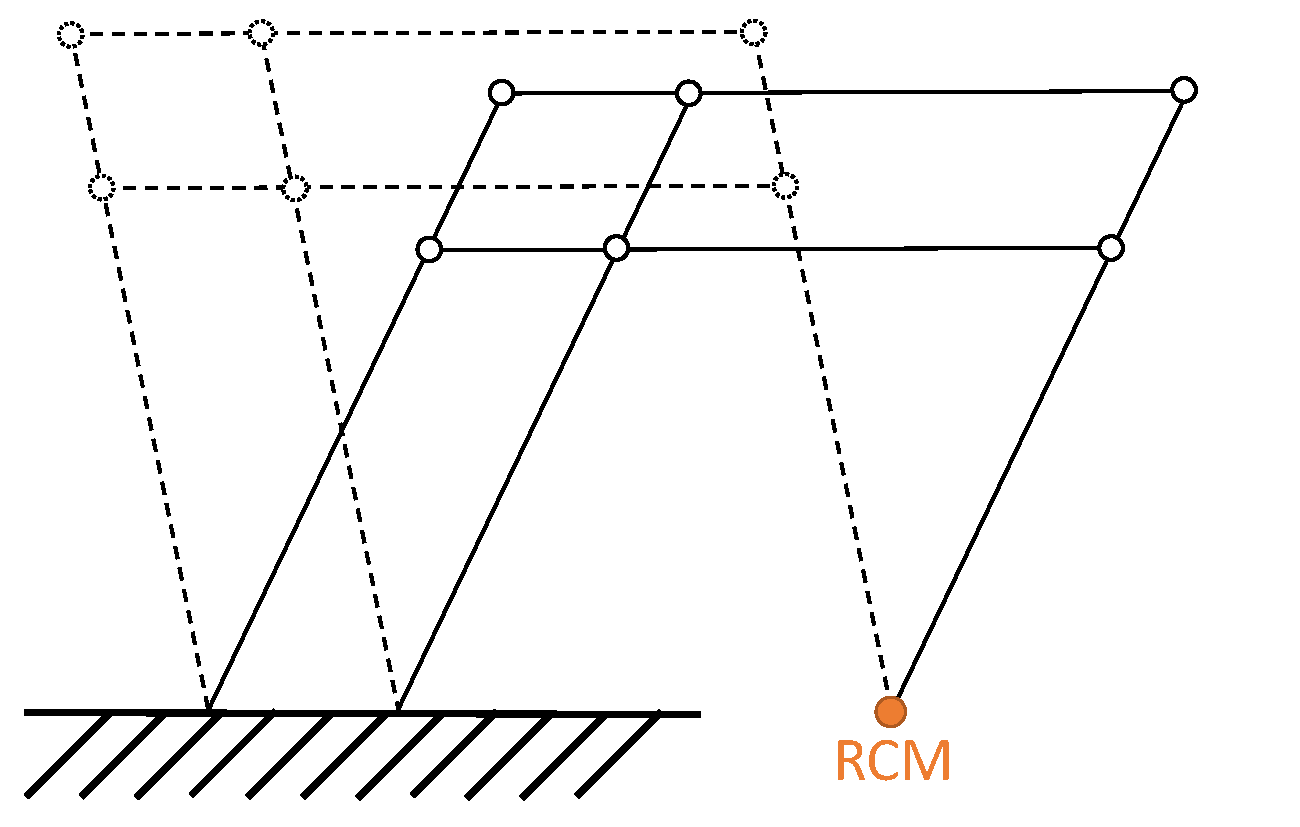
\includegraphics[width=6cm]{mechRCM}
	\caption{A simple, parallelogram based RCM mechanism. The RCM point is mechanically constrained and cannot move relative to the base frame of the robot.}
	\label{mechRCM}
\end{figure}
\begin{figure}[b!]
	\centering
	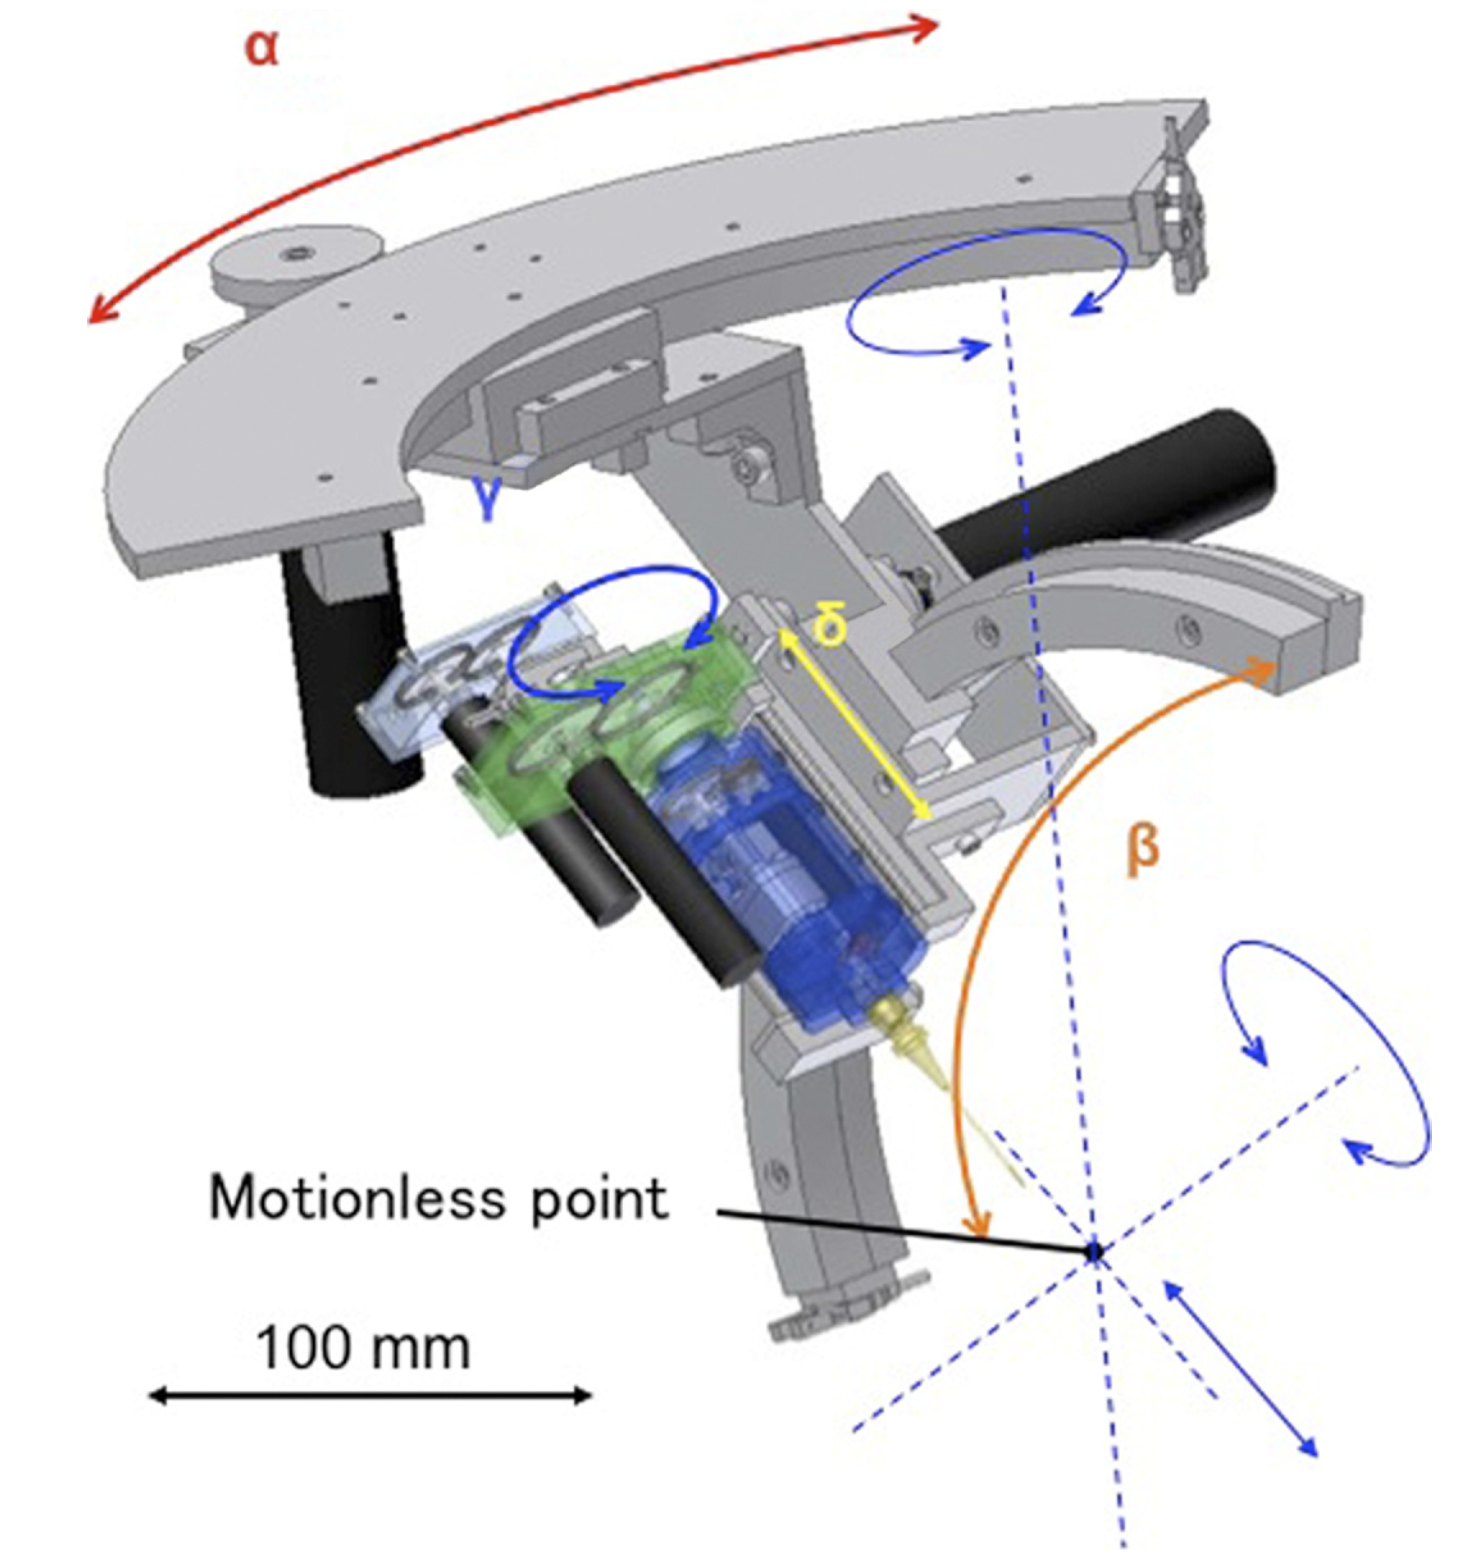
\includegraphics[width=7cm]{Ueta2017_robot}
	\caption{A mechanically constrained robot for ophthalmic surgery developed at the University of Tokyo \cite{Ueta2017}.}
	\label{Ueta2017img}
\end{figure}

Introduction of robots to clinical practice brings several benefits. One major point of interest is to provide smooth, tremor-free position control and force scaling for the tool. Robotic assistance seems especially promising in ophthalmic surgery, which relies on high precision to prevent damage to the delicate tissue of the eye. To minimize damage on the surrounding tissue, movement of the tool laterally to the point of incision must be prevented. While this is a challenging task for a surgeon it is comparably easy for a robot. This concept is referred to as Remote Center of Motion (RCM) and generally divided into two subcategories: \textbf{mechanically constrained} and \textbf{programmable} RCM. 

Examples for a mechanically constrained RCMs are shown in Figures \ref{mechRCM} and \ref{Ueta2017img}. Here, the RCM point is always in the same position relative to the base frame. Mechanically constraining the RCM point is superior in precision and reliability but offers little flexibility in ophthalmic surgery since the position of the robot defines the motionless point and consequently the patient or the whole robot need to be moved until the RCM point coincides with the point of incision.

A programmable RCM, sometimes referred to as a \textit{virtual fixture} \cite{MingLi2004}, is achieved by algorithmically forcing the velocity of an arbitrary point on the manipulator to be zero. This significantly increases the flexibility of the system, but also increases the complexity of the controller required to maintain high precision. Furthermore, a programmable RCM point is in general considered to be less safe than mechanically constrained systems.

The iRAM!S project \cite{nasseri2013introduction} is a joint collaboration of the informatics institute \textit{Robotics and Embedded Systems}, the Graduate School of Information Science in Health (GSISH) and the TUM university hospital Klinikum rechts der Isar. The goal of the project is the development of a novel robotic system for assisting ophthalmic surgeons in complex retinal surgeries, for example for the treatment of diseases such as retinal vein occlusion.

\begin{figure}[t!]
	\centering
	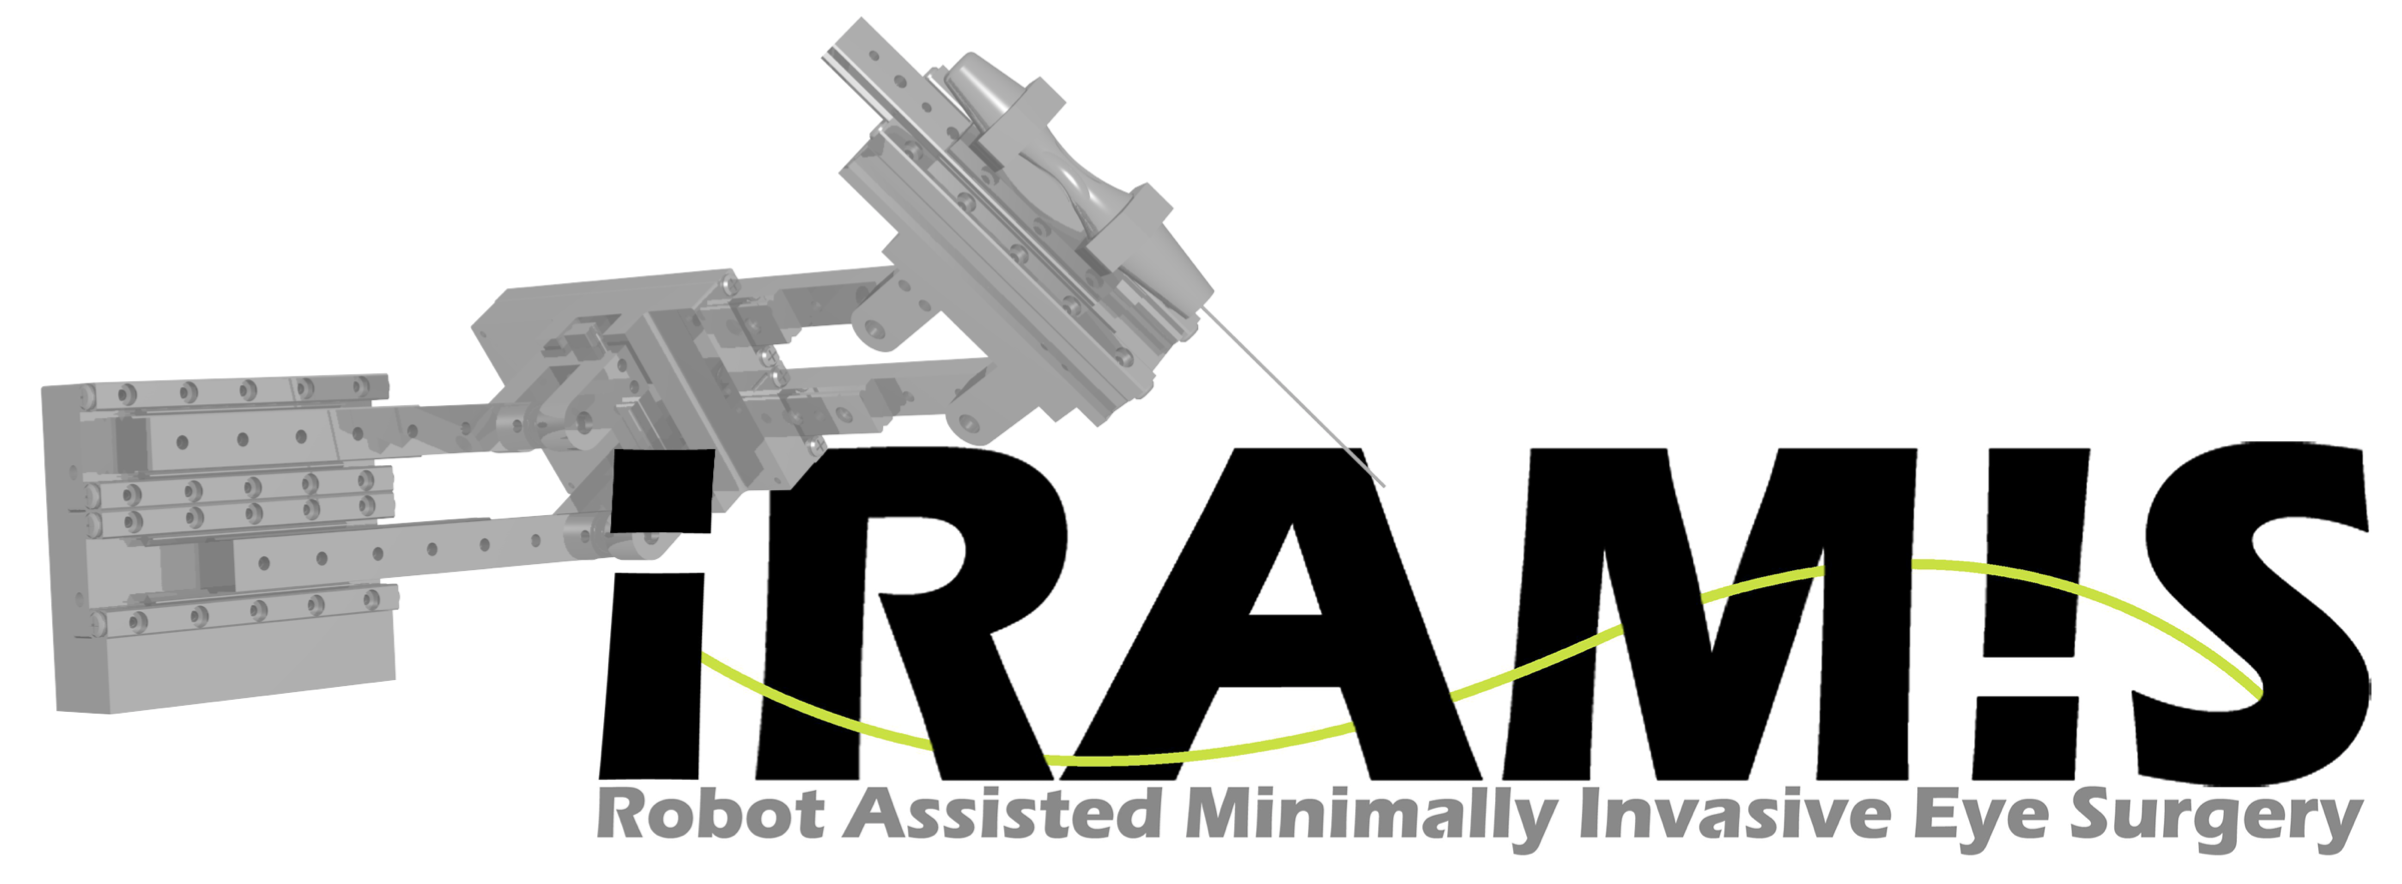
\includegraphics[width=12cm]{iRAM!S}
	\caption{The robotic assistant for ophthalmic surgery developed within the iRAMI!S project \cite{iramis}.}
	\label{iRAM!S}
\end{figure}

\section{Outline}
The second chapter of this thesis describes the mechanical design of the robot and reviews the kinematic relations between joint movements and end effector pose. A step by step description is presented on how to derive the Jacobian from the Denavit-Hartenberg parameters of the robot. 

The Jacobian pseudoinverse approach as a solution for the inverse kinematics problem is introduced, along with the concept of the \textit{augmented Jacobian matrix}, which is used to implement the Remote Center of Motion constraint. Finally, there is a brief introduction to the simulation environment V-REP which will be used to validate the results of the thesis.

In the third chapter, the extended robot task and corresponding Jacobian matrix is defined. A V-REP simulation model is designed from the CAD file and controlled both via a MATLAB remote API and a child script using V-REPs built-in inverse kinematics function. 

In the final Section, the precisions and execution times of both methods are evaluated and compared.
\chapter{Background}

In this chapter, the mechanical design and kinematic relationships of the surgical robot developed in the iRAMs! project will be reviewed. The Jacobian matrix and the Jacobian pseudoinverse approach are presented as an iterative solution to the inverse kinematics problem. Lastly, there is a short introduction to the V-REP simulation environment and the Dampened Least Squares method used by V-REPs internal inverse kinematics solver. 

\section{Mechanical Design}
\begin{figure}[b!]
	\begin{center}
		%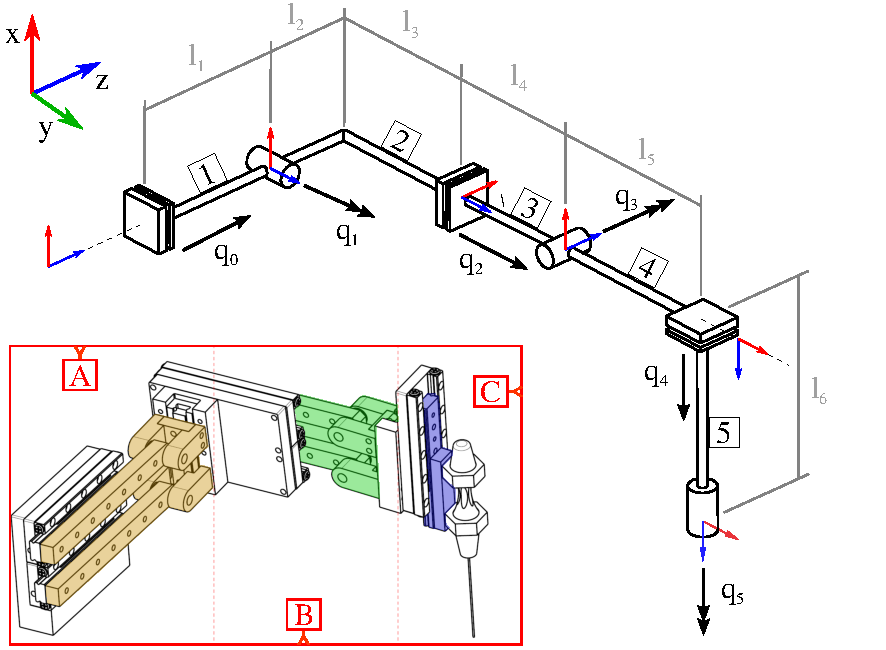
\includegraphics[width=15cm]{manipulator_overview_refactored}
		\import{images/}{manipulator_overview_refactored_tex.pdf_tex}
		\caption{The simplified serial manipulator, consisting of two subsequent PCJM elements (A and B) and a simple prismatic stage (C). Each PCJM element can be modelled as a translation and a following rotation. Adapted from \cite{Master_thesis}.}
		\label{Manipulator}
	\end{center}
\end{figure}

The surgical robot considered in this thesis consists of two subsequent \textit{Parallel Coupled Joint Mechanisms} (PCJMs), one single prismatic joint and one optional revolute joint, providing six degrees of freedom.

Each PCJM consists of two stick-slip piezo actuators moving parallel to each other at a distance \textit{d}. 
Translating both sliders the same distance results in a pure translation of the manipulator, while a differential movement results in an additional rotation. In contrast to a linear chain of prismatic and revolute joints, the PCJM approach provides higher stiffness and precision. 

\begin{figure}[t!]
	%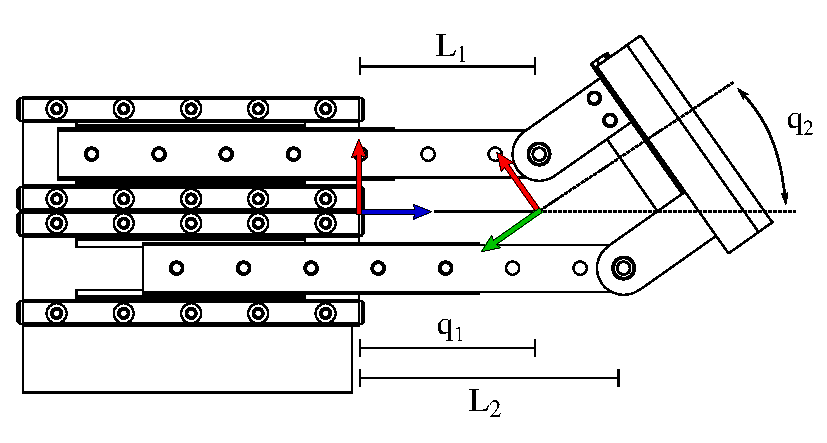
\includegraphics[width=\textwidth]{pcjm}
	\import{images/}{pcjm_refactored_tex.pdf_tex}
	\caption{A single Parallel Coupled Joint Mechanism. Differential displacement of the two prismatic joints $L_1$ and $L_2$ results in both a translation and rotation of the subsequent link. Adapted from \cite{Ali_FK}.}
	\label{pcjm}
\end{figure}

For a simpler kinematic analysis, the PCJM elements can be treated as a prismatic and subsequent revolute joint.
The two translations $L_1$ and $L_2$ correspond to the translation of the prismatic joint $q_0$ and angle of the revolute joint $q_1$ as
\begin{eqnarray}
	q_0	&=&	\frac{L_1+L_2}{2} \\
	q_1	&=&	\arctan(\frac{L_2-L_1}{d})\;.
\end{eqnarray}

Conversely, given the two joint positions $q_0$ and $q_1$, the slider positions can be uniquely determined via: 
\begin{eqnarray}
	L_1	&=&	\frac{d\cdot \tan(q_1)}{2}+q_0 \\
	L_2	&=& 2 q_0-L_1\;.
\end{eqnarray}


\section{Forward Kinematics}\label{FK}

In order to describe the position of the end effector relative to the base coordinate frame we determine the Denavit-Hartenberg parameters \cite{hartenberg} of the robot. First, a coordinate system is placed in each joint according to the following rules:
\begin{itemize}
	\item The z-axis must point along the axis of rotation or translation of the joint.
	\item The x-axis for the base frame is a free choice. For each subsequent joint, the x-axis is co-linear with the common normal of the current and previous z-axis, with its origin at the intersection with the new z-axis.  $x_n=z_n\times z_{n-1}$. The origin of the new coordinate system is not necessarily in the center of the joint.
	\item The y-axis is chosen so that it forms a right handed coordinate system with x and z.
\end{itemize}
Figure \ref{Manipulator} illustrates the placement of the coordinate systems for each joint. 
Having established the coordinate systems, we can now determine the Denavit-Hartenberg parameters $d_i$, $\theta_i$, $a_i$ and $\alpha_i$:
\begin{itemize}
	\item $d_i$ is the depth of origin $i$ to origin $i-1$ along the previous z-axis $z_{i-1}$. 
	\item $\theta_i$ is the angle about the previous z axis $z_{i-1}$ to align $x_{i-1}$ with the new origin $i$.
	\item $a_i$ is the distance between the current and previous origin along the previous rotated x-axis $x_{i-1}$.
	\item $\alpha_i$ is the angle between $z_{i-1}$ and $z_i$ along the current x-axis $x_i$.
\end{itemize}

We can now determine the homogeneous transformation that describes the position of each coordinate frame with respect to the preceding one. For each link $i$, the transformation from link $i-1$ to link $i$ is given by:
\begin{equation}\label{T_i}
T_{i-1}^i=\begin{bmatrix}
		\cos\theta_i & -\sin\theta_i\cos\alpha_i & \sin\theta_i\sin\alpha_i & a_i\cos\theta_i \\
		\sin\theta_i & \cos\theta_i\cos\alpha_i & -\cos\theta_i\sin\alpha_i & a_i\sin\theta_i\\
		0 & \sin\alpha_i & \cos\alpha_i & d_i\\
		0 & 0 & 0 & 1
		\end{bmatrix}\\
		\\
\end{equation}
Table \ref{parameters} shows the values obtained for the Denavit-Hartenberg parameters. The values for the link lengths $l_i$ are obtained from the CAD model. 

The transformation from the origin to the end effector can now be obtained by subsequently multiplying the transformation matrices of each subsequent coordinate fame pair:
\begin{eqnarray}\label{Pi_6}
	T_0^6 &=& \Pi_{i=1}^6 T_{i-1}^i
\end{eqnarray}

% use \matminus instead of -
%			-s1s5-c1c5s3 & c1s3s5-c5s1 & -c1c3 & l2s1-c1c3(q4+l6)-l5c1s3 \\
%			c3c5 & -c3s5 & -s3 & l3+l4+q2-s3(q4+l6)+l5c3\\
%			c5s1s3-c1s5 & -c1c5-s1s3s5 & c3s1 & l1+q0+l2c1+c3s1(q4+l6)+l5s1s3\\
%			0 & 0 & 0 & 1

\begin{equation}\label{T_6}
=	\begin{bmatrix}
			\matminus s1s5\matminus c1c5s3 & c1s3s5\matminus c5s1 & \matminus c1c3 & l2s1\matminus c1c3(q4\matplus  l6)\matminus l5c1s3 \\
			c3c5 & \matminus c3s5 & \matminus s3 & l3\matplus  l4\matplus  q2\matminus s3(q4\matplus  l6)\matplus  l5c3\\
			c5s1s3\matminus c1s5 & \matminus c1c5\matminus s1s3s5 & c3s1 & l1\matplus  q0\matplus  l2c1\matplus  c3s1(q4\matplus  l6)\matplus  l5s1s3\\
			0 & 0 & 0 & 1
	\end{bmatrix}
\end{equation}
with $ci,si := \cos(i), \sin(i)$, where the $3\times 3$ matrix in the upper left describes the rotation of the tool relative to the base frame while the $3\times 1$ vector in the upper right describes the position of the needle tip with respect to the base coordinate system and will be denoted as $O_6(q)$.

\begin{table}[h!]
\centering
 \begin{tabular}{|c|c|c|c|c|}
 	\hline
    Link & $\theta_i$ & $d_i$ & $a_i$ & $\alpha_i$\\
    \hline
    1 & 0 & $q_0+l_1$ & 0 & $-\frac{\pi}{2}$\\
    2 & $q_1-\frac{\pi}{2}$ & $l_3$ & $l_2$ & 0\\
    3 & $\frac{\pi}{2}$ & $l_4+q_2$ & 0 & $\frac{\pi}{2}$\\
    4 &$\frac{\pi}{2}+q_3$ & 0 & $l_5$ & $-\frac{\pi}{2}$\\
    5 & 0 & $l_6+q_4$ & 0 & 0\\
    6 & $q5$ & 0 & 0 & 0\\
    \hline
 \end{tabular}
 \begin{tabular}{|c|c|}
 	\hline
    Offset & [mm]\\
    \hline
    $l_1$ & $71$\\
    $l_2$ & $33.5$\\
    $l_3$ & $-23$\\
    $l_4$ & $71$\\
    $l_5$ & $28$\\
    $l_6$ & $97$\\
    \hline
 \end{tabular}
 \caption{The Denavit-Hartenberg parameters of the serial robot. A negative value for a link length is the result of the choice for the origin of a coordinate system within a PCJM and will not lead to an error in subsequent computations.}\label{parameters}
\end{table}

\section{Inverse Kinematics}\label{section_IK}

The forward kinematics relation gives information about how the position and orientation of the end effector will change with a change in joint positions. Each distinct joint vector $\bm{\theta} = (q_1,q_2,...,q_5)$ leads directly to the pose of the end effector as determined by Eqn. \ref{T_6}. It follows that in order to control the pose of the needle we need to consider the inverse problem, that is, finding a set of joint variables for a desired end effector pose. The inverse kinematics problem is, in general, more difficult to solve, may not always have a unique or best solution or be guaranteed to have a closed form equation for the solution. The Jacobian matrix provides an iterative solution to the inverse kinematics problem.

\subsection{The Jacobian Matrix and the Jacobian Pseudoinverse}

With the Jacobian matrix we want to relate the linear and angular velocity of the end effector $\dot{x}$ to the vector of joint velocities $\dot{\bm{\theta}}(t)$. It is a function of the joint angles defined by

\begin{eqnarray}
	J(\bm{\theta}) &=&(\frac{\partial x_i}{\partial\theta_j})_{i,j} \; ,
\end{eqnarray}
with $J \in \mathbb{R}^{m\times n}$, m: degrees of freedom, n: number of links.
 
According to \cite{textbookJacobian}, each column of the Jacobian matrix can be calculated independently using  the Denavit-Hartenberg parameters as follows:
\begin{eqnarray}
	J_0^n=[J_1,J_2,... ,J_n]
\end{eqnarray}
where $n$ is the number of links. For this robot $n=6$.

In case joint $i$ is a revolute joint $J_i$ is given by
\begin{eqnarray}\label{i_revolute}
	J_i=	\begin{bmatrix}
			Z_{i-1}\times(O_n-O_{i-1})\\
			Z_{i-1}
		\end{bmatrix}	
\end{eqnarray}
and in case of a prismatic joint
\begin{eqnarray}\label{i_prismatic}
	J_i=	\begin{bmatrix}
			Z_{i-1}\\
			0
		\end{bmatrix}	
\end{eqnarray}
where $Z_i$ and $O_i$ are composed of the first three elements of the third and fourth column in $T_0^i$, respectively. Using Eqns.\ref{T_i}, \ref{Pi_6}, and Table \ref{parameters}, the Jacobian matrix for every link with respect to the base coordinate frame can be calculated. For the full transformation from the base to the end effector this results in:
\begin{eqnarray}\label{J_6}
	J_0^6=\begin{bmatrix}	
				0 & l2c1\matplus l6c3s1\matplus l5s1s3\matplus q4c3s1 & 0 & c1(l6s3\matminus l5c3\matplus q4s3) & \matminus c1c3 & 0\\
				0 & 0 & 1 & \matminus l6c3\matminus l5s3\matminus q4c3 & \matminus s3 & 0\\
				1 & l6c1c3\matminus l2s1\matplus l5c1s3\matplus q4c1c3 & 0 & \matminus s1(l6s3\matminus l5c3\matplus q4s3) & c3s1 & 0\\
				0 & 0 & 0 & s1 & 0 & \matminus c1c3\\
				0 & 1 & 0 & 0 & 0 & \matminus s3\\
				0 & 0 & 0 & c1 & 0 & c3s1\\
			\end{bmatrix}
\end{eqnarray}

Since the tool used by the surgical robot in this thesis is a straight needle, the rotation about the needle axis $q_5$ has no effect on the end effector pose. Thus for the derivation of the extended Jacobian matrix, only the transformation from the base frame to the needle tip, without the final revolute joint will be considered:
\begin{eqnarray}\label{J_5}
J_0^5 =	\begin{bmatrix}	
		0 & l2c1\matplus l6c3s1\matplus l5s1s3\matplus q4c3s1 & 0 & c1(l6s3\matminus l5c3\matplus q4s3) & \matminus c1c3\\
		0 & 0 & 1 & \matminus l6c3\matminus l5s3\matminus q4c3 & \matminus s3\\
		1 & l6c1c3\matminus l2s1\matplus l5c1s3\matplus q4c1c3 & 0 & \matminus s1(l6s3\matminus l5c3\matplus q4s3) & c3s1\\
		0 & 0 & 0 & s1 & 0\\
		0 & 1 & 0 & 0 & 0\\
		0 & 0 & 0 & c1 & 0\\
		\end{bmatrix}
\end{eqnarray}

Lastly, we need to check if there are any singularities of $J^5_0$ within the workspace of the robot. This can be done by taking a look at the determinant of the Jacobian matrix which is 
\begin{eqnarray}\label{det_J_5}
	det(J^5_0) &=& \cos(q_1)\;\cos(q_3)^2\; .
\end{eqnarray}
It can only reach zero if either $q_1$ or $q_3$ are zero, which is not a possible configuration for the robot.

Given a vector of joint velocities $\bm{\dot{\theta}}$, the vector of end effector velocities is given by
\begin{eqnarray}
	\bm{\dot{x}}&=&J(\bm{\theta}) \; \bm{\dot{\theta}} \;.
\end{eqnarray} 
This relationship is now used as an iterative solution to the inverse kinematics problem. For some error $\bm{e}$ between the current and target end effector pose, we seek to find an update value $\Delta\bm{\theta}$ for the joint angles such that the change in end effector positions is equal to the error $\bm{e}$.
\begin{eqnarray}\label{Jac_approx}
	\bm{e} = \Delta \bm{x} \approx J(\bm{\theta}) \; (\bm{\theta} + \Delta\bm{\theta})
\end{eqnarray}
To obtain a good estimate for $\Delta\bm{\theta}$ we employ the Moore-Penrose Pseudoinverse of $J$, $J^{\dagger}$
\begin{eqnarray}\label{J_pseudo}
	\Delta\bm{\theta} = J^{\dagger}(\bm{\theta}) \; \bm{e}
\end{eqnarray}
The resulting vector $\Delta\bm{\theta}$ is the unique vector of smallest magnitude which minimizes\\ 
 $||J\Delta\bm{\theta} = \bm{e}||$ \cite{iksurvey}.
The Jacobian matrix only provides an approximation of the actual change in end effector pose because it is a function of $\bm{\theta}$. For small errors, the change in joint positions is small enough for $J$ to be roughly constant and $\Delta \bm{x}$ to be a good approximation to $\bm{e}$. If the error between the current and desired end effector pose is large, we use an iterative approach:
\begin{itemize}
	\item Calculate the Jacobian matrix from the current joint positions $\bm{\theta}$ and compute $J^{\dagger}$.
	\item Obtain an update $\Delta\bm{\theta}$ for small step of predetermined magnitude towards the goal pose using Eqn. \ref{J_pseudo}.
	\item Repeat with the new joint positions $\bm{\theta} + \Delta\bm{\theta}$ until the pose is sufficiently close to the target pose.
\end{itemize}

Finally, it is important to note that the Jacobian pseudoinverse method is often plagued by numeric instability near singularities where $J$ is rank deficient, resulting in large values for $\Delta\bm{\theta}$ \cite{J_stability}. However, since the Jacobian matrix of the surgical robot has no singularities within its workspace, this is not an issue for this thesis. 

\section{The V-REP Simulation Environment}

\subsection{Introduction to V-REP}

In order to verify and evaluate the kinematic relations established in the previous section, the movement of the robot is simulated using V-REP\cite{vrep}. 
V-REP is a general purpose robot simulator with an integrated development environment distributed by Coppelia Robotics \cite{coppelia}. A V-REP simulation or \textit{simulation scene} consists of several different \textit{scene objects} that are assembled in a \textit{scene hierarchy} with each element having exactly one parent element and a variable amount of child objects. The objects relevant for our purposes are: 
\begin{itemize}
\item \textbf{Shape:} Any rigid body (e.g. a link of the surgical robot), represented by a triangle mesh. There are different types of shapes supported by V-REP: \textit{pure} shapes (e.g. spheres, cuboids), \textit{convex} shapes and \textit{random} shapes, which are neither pure nor convex. All shapes used in this simulation are random shapes, since no collision detection or dynamic calculation will be performed that would benefit from modelling the robot using simple shapes with a lower triangle count.
\item \textbf{Joint:} A joint object constrains how two \textit{scene objects} move relative two each other. In the scene hierarchy, a joint will be placed as a child of the first object and parent of the second object. Relevant for this model are revolute joints (rotation about one axis) and prismatic joints (translation along one axis).
\item \textbf{Dummy:} A dummy object has no physical properties or dimensions, it is used as a 'helper object'. In the surgical needle model, it is used to introduce different frames of reference on the same link, for example at the base, RCM point and tip of the needle. Dummy objects are also used as \textit{tip} and \textit{target} objects for kinematic and dynamic calculations. 
\item \textbf{Graph:} A graph object records a given data stream and may directly display it. For the surgical robot, a graph object is attached to the RCM point and tip of the needle to record its position over time. 
\end{itemize}

The model can be controlled either by a remote API or an embedded child script. For this thesis, all communication with the simulation is carried out by MATLAB \cite{MATLAB} scripts. Using the V-REP remote API functions \cite{remoteAPI}, the pose of all simulation objects can be received and modified. 

The V-REP inverse kinematics module handles IK resoultion via \textit{IK groups} consisting of a number of \textit{IK elements}, one for each constraint that needs to be fulfilled simultaneously. For the surgical robot, one IK group consiting of two IK elements is needed: the first element is responsible for placing the needle tip within the eye, the other for fixing the RCM point at the trocar entry. Each IK element is made up of a \textit{tip-target dummy pair}: The 'tip' dummy is placed on the robot while the 'target' dummy can be placed anywhere in the workspace of the robot. Once the simulation is started, each 'tip' dummy will automatically try to converge to its corresponding 'target' dummy. The position of the two target dummies, one for the tip and one for the RCM, can then be controlled by the MATLAB script.

\subsection{Dampened Least Squares}\label{DLS}

The V-REP inverse kinematics solver uses a Dampened Least Squares (DLS) method, also referred to as the Levenberg-Marquardt algorithm (LMA) \cite{levenberg, marquardt}. It is a method to solve nonlinear least squares problems and can be seen as a mixture of the Gauss-Newton method and standard gradient descent \cite{bjorck}. As explained in  Section \ref{section_IK}, the inverse kinematics problem is to find a value for $\Delta\bm{\theta}$ which minimizes the error in the pose  $\bm{e}=J(\bm{\theta}) \; \Delta\bm{\theta}$. The Jacobian pseudoinverse method minimizes this quantity by setting $\Delta\bm{\theta}=J^{\dagger}(\bm{\theta}) \; \bm{e}$, which gives an optimal solution in the sense of least squares but is numerically unstable near singularities. The DLS algorithm instead minimizes 
\begin{eqnarray}\label{dampened}
	||J\Delta\bm{\theta}-\bm{e}||^2 + D^2||\Delta\bm{\theta}||^2,
\end{eqnarray} 
where D is the non-zero \textit{damping constant}.
It was shown in \cite{DLS_theta} that the minimum of Eqn. \ref{dampened} can be expressed as
\begin{eqnarray}\label{f}
	\Delta\bm{\theta} &=& J^T(J \, J^T+D^2I)^{-1}\bm{e}\;.
\end{eqnarray}
One large advantage of Eqn. \ref{f} is that the matrix inversion never has to be explicitly computed, instead a vector $\bm{f}$ can be found through row operations such that
\begin{eqnarray}\
	(J \, J^T+D^2I)^{-1}\bm{f} &=&\bm{e}\;. 
\end{eqnarray} 
Then, the DLS solution is given by $J^T\bm{f}$.
One important choice is the value of the damping constant $D$. A larger value of $D$ corresponds to more stable behaviour near singularites but reduces the convergence rate. Methods for choosing and adapting $D$ based on the configuration of the robot are proposed for example in \cite{D2} and \cite{D1}.
\chapter{Method}
In the first part of this chapter, the concept of the augmented Jacobian matrix is introduced. In this approach, the redundancy of the robot is used to define the additional kinematic task of maintaining a remote center of motion. The resulting composite Jacobian matrix can then be used to simultaneously control the position of the tool tip within the eye and prevent movement of the needle at the point of incision. A method for estimating the precision of the augmented Jacobian matrix is proposed. The second part of this chapter describes the transfer of the CAD model of the robot into a V-REP simulation model and explains how to adapt the model in order to be usable by the built-in inverse kinematics solver. 

\section{Remote Center of Motion Constraint}
After entry into the eye via the trocar, the movement of the tool is further constrained. In order to minimize damage on the surrounding tissue, the needle may only translate along its own axis or rotate about the entry point.

When moving the needle outside of the eye, we care about the position of the tool tip, but not necessarily about its orientation. For each position of the tool tip, there are infinitely many ways in which the other links can be arranged in order to reach the desired end effector position, the manipulator is \textit{redundant}.
Disregarding the rotation about the tool axis, the robot has $n=5$ degrees of freedom. $m=3$ degrees of freedom are needed to control the position of the tool tip. Now let $r=n-m$ be the degree of 'redundancy'. Following the approach presented in \cite{augmentedJacobian}, a set of \textit{r} task-related kinematic functions,
\begin{eqnarray}
	\bm{\Phi} &=& \{\phi_1(\bm{\theta}),...\; ,\phi_r(\bm{\theta})\} \; ,
\end{eqnarray}
can be formed to describe the variation of these remaining degrees of freedom and define an additional task for the robot. The choice of these functions is somewhat arbitrary, yet there are some choices that produce algorithmic singularities (discussed at the end of this section).

By then specifying a set of end effector position coordinates,\begin{eqnarray}
	\bm{Y} &=& \{y_1(\bm{\theta}),...\; ,y_m(\bm{\theta})\} \; ,
\end{eqnarray}
and a set of kinematic functions $\bm{\Phi}$, for each robot task there is a unique solution for the joint positions. Both the kinematic functions and the end effector coordinates can be combined to provide a set of generalized \textit{configuration variables} for the manipulator,
\begin{eqnarray}
	\bm{X} &=& \{\bm{Y},\bm{\Phi} \} = \{y_1(\bm{\theta}),...\; ,y_m(\bm{\theta}) \; \vdots  \;\phi_1(\bm{\theta}),...\; ,\phi_r(\bm{\theta})\} \\
	&=& \{x_1(\bm{\theta}),...\; ,x_n(\bm{\theta})\} \; .
\end{eqnarray}
We obtain the \textit{augmented forward kinematic model} which relates the configuration vector $\bm{X}$ to the joint angles $\bm{\theta}$ via the \textit{augmented Jacobian matrix} $J_a(\bm{\theta})$. 

\begin{eqnarray}
	\bm{\dot{X}}(t) &=& J_a(\bm{\theta}) \dot{\bm{\theta}} \; ,
\end{eqnarray}
where 
\begin{eqnarray}
	J_a(\bm{\theta})=
		\begin{bmatrix}
			J_e(\bm{\theta})\\[3pt]
			J_c(\bm{\theta})
		\end{bmatrix}	
				=
		\begin{bmatrix}
			\frac{\partial \bm{Y}}{\partial \bm{\theta}}\\[3pt]
			\frac{\partial \bm{\Phi}}{\partial \bm{\theta}}\\
		\end{bmatrix} \; .
\end{eqnarray}
					
Is the $n \times n$  augmented Jacobian matrix, consisting of $J_e \in  \mathbb{R}^{m\times n}$, that is related to the motion of the end effector and $J_c \in  \mathbb{R}^{r\times n}$ related to the additional kinematic task.			
This accomplishes \textit{simultaneous} control of end effector motion as well as utilizing the redundancy to achieve an additional task.

The procedure for the calculation of the extended Jacobian Matrix has already been presented in \cite{AliRCM} and will be reviewed in this thesis.   
In this setup, the additional kinematic task is to force the velocity of a point $\bm{p}_{rcm}$ on the needle to zero.
The remote center of motion is assumed to be on the axis of the tool and can be written as:
\begin{eqnarray}
	\bm{\Phi} &=& \bm{p}_{rcm} = \bm{p}_{base}+\lambda(\bm{p}_{tip}-\bm{p}_{base}) \; ,
\end{eqnarray}
with $\bm{p}_{rcm}$, $\bm{p}_{base}$, and $\bm{p}_{tip} \in \mathbb{R}^{3\times1}$ and $\lambda \in \mathbb{R}^{1\times1}$. 

\begin{figure}[t!]
	\begin{center}
		%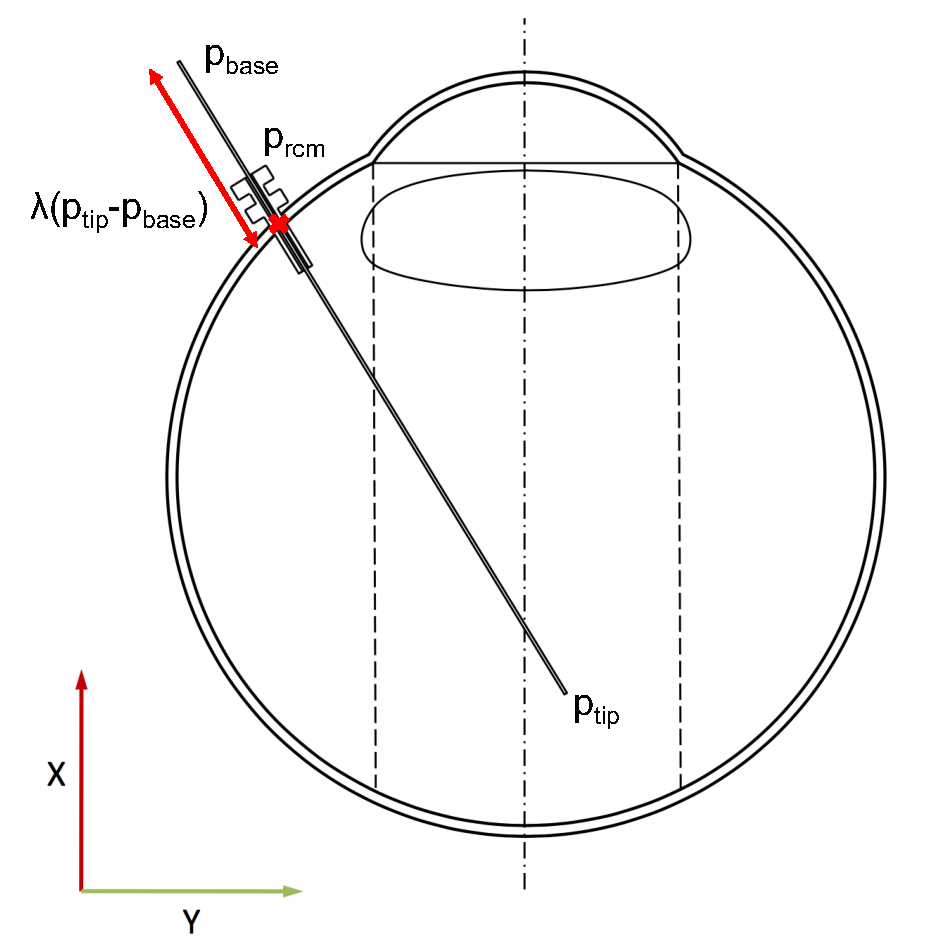
\includegraphics[width=120pt]{lambda}
		\import{images/}{lambda_refactored_tex.pdf_tex}
		\caption{Location of $\bm{p}_{rcm}$}
		\label{lambda}
	\end{center}
\end{figure}

Differentiating with respect to time:
\begin{eqnarray}
	\bm{\dot{p}}_{rcm} = \bm{\dot{p}}_{base}+\lambda(\bm{\dot{p}}_{tip} - \bm{\dot{p}}_{base})+\dot{\lambda}(\bm{p}_{tip} - \bm{p}_{base})
\end{eqnarray}

As previously established, the change in position of any link $i$ can be described as $p_i = J_i q_i$ and thus:
\begin{eqnarray}
	\bm{\dot{p}}_{rcm}=J_{base}\bm{\dot{\theta}}+\lambda(J_{tip}\bm{\dot{\theta}}-J_{base}\bm{\dot{\theta}})+\dot{\lambda}(\bm{p}_{tip}-\bm{p}_{base}) \; ,
\end{eqnarray}
where $J_{base}$ and $J_{tip}$ are the Jacobian matrices corresponding to point $\bm{p}_{base}$ and $\bm{p}_{tip}$ respectively. $J_{tip}$ describes the linear velocity of the tool tip, disregarding the rotation around its own axis ($q_5$). Hence, $J_{tip}$ is equal to the top three rows of $J_0^5$ calculated in the previous section. The points $\bm{p}_{tip}$ and $\bm{p}_{base}$ are on the same rigid link, only at a different distances to he previous joint. Thus, $J_{tip}$ can be modified to describe the motion of point $\bm{p}_{base}$ by substituting $l_6$ with 0, yielding $J_{base}$.
$\bm{\dot{p}}_{rcm}$ can be expressed in matrix form as: 
\begin{eqnarray}
	\bm{\dot{p}}_{rcm} =
		\begin{bmatrix}
			J_{base}+\lambda(J_{tip}-J_{base}) \\[2pt]
			\bm{p}_{tip} - \bm{p}_{base}
		\end{bmatrix}^T
		\begin{bmatrix}
			\bm{\dot{\theta}} \\[2pt]
			\dot{\lambda}
		\end{bmatrix}
	= J_{c}
		\begin{bmatrix}
			\bm{\dot{\theta}} \\[2pt]
			\dot{\lambda}
		\end{bmatrix} 
	= J_{c} \; \bm{\dot{\theta}}_{ext} \; ,
\end{eqnarray}			
with $\bm{\dot{p}}_{rcm} \in \mathbb{R}^{3\times1}$,  $J_{tip}$, $J_{base} \in \mathbb{R}^{3\times5}$ and $J_{c} \in \mathbb{R}^{3\times6}$. The set of extended joint angles $\bm{\theta}_{ext}$ are given as 
\begin{eqnarray}
	\bm{\dot{\theta}} & = & \{ q_1,... \, , q_5, \lambda \} \; .
\end{eqnarray}
Now we can enforce the remote center of motion constraint by setting the velocity of the RCM point to zero. That is, $\bm{p}_{rcm}$ should not change its position.
\begin{eqnarray}
	\bm{\dot{p}}_{rcm}	= J_{c}
			\begin{bmatrix}
				\bm{\dot{q}} \\[2pt]
				\dot{\lambda}
			\end{bmatrix}
					= 0^{3\times 1}
\end{eqnarray}

Hence we have defined the additional kinematic task $\bm{\Phi} = \{x_{rcm}, y_{rcm}, z_{rcm}\}$ and its associated Jacobian $J_c$ in Cartesian coordinates with respect to the robot base frame. 
Although forcing $\bm{\dot{p}}_{rcm}$ to be zero is a constraint of dimension three, modelling the variation of $\lambda$ increases the degrees of freedom by one. Hence, $r=2$ degrees of freedom are lost due to the RCM constraint and $m=3$ degrees of freedom remain to place the tool tip within the eye. 
We choose a set of variables $\bm{Y}$ to represent the position of the end effector that doesn't introduce algorithmic singularities. 
\begin{eqnarray}
	\bm{Y} &=&	\{ x, \phi, \psi\} \; ,
\end{eqnarray}
where $x$ is the global x-position of the tool tip and $\phi$ and $\psi$ describe the angle of the tool.
$\bm{Y}$ and $\bm{\Phi}$ can now be combined to form a set of generalized kinematic functions for the end effector performing the extended task,
\begin{eqnarray}
	\bm{X}_{ext} &=& \{x, \phi, \psi, x_{rcm}, y_{rcm}, z_{rcm} \} \; ,
\end{eqnarray}
and the associated augmented Jacobian
\begin{eqnarray}
	J_{a} =
		\begin{bmatrix}
			J_e \hspace{10pt} 0_{3 \times 1} \\[3pt]
			J_c
		\end{bmatrix}	
		=
		\begin{bmatrix}
			\frac{\partial \bm{Y}}
				{\partial \bm{\theta}} \\[3pt]
			\frac{\partial \bm{\Phi}}
				{\partial \bm{\theta}}
		\end{bmatrix}
\end{eqnarray}
where $J_e$ is the Jacobian matrix relating the end effector x-position and tool angles $\phi $ and $\psi$ to the joint positions. Thus, $J_e$ is composed of the first, fifth, and sixth row of $J_{base} \in \mathbb{R}^{3\times5}$.

Lastly, we need to check if there are any singularities within $J_a$, i.e. if the kinematic functions we chose have any dependencies. One has to differentiate between kinematic and algorithmic singularities. Kinematic singularities refer to any configurations in which $J_e$ is rank deficient, e.g. when two links joined by a revolute joint become co-linear. It was previously established that this is not possible due to the mechanical design of the robot. Algorithmic singularities are introduces by the choice of the kinematic functions $\bm{\Phi}$, if $J_c$ in itself is rank-dependent or if two rows of $J_e $ and $J_c$ are linearly dependent. For the presented case the determinant
\begin{eqnarray}
	det(J_a) &=&	-l_6\cos(q_1)^2\cos(q_3)^2\sin(q_1) \; ,
\end{eqnarray}
is only zero for $q_3 = \pm\frac{\pi}{2}$, which is not a reachable configuration. $J_a$ is listed as Eqn. \ref{J_a_full} in the Appendix.\\

\section{Controller Design}

Having established the augmented Jacobian matrix we can now compute the change in joint position necessary to achieve a certain change in end effector position. However, iteratively using $\Delta \bm{\theta}=J^{\dagger}\Delta \bm{x}$ often does not result in a smooth trajectory from the current to the target pose. If for example the target pose differs from the current pose in only one angle, the Jacobian matrix will return a vector Q correcting the error in angle by rotating the needle. in the next iteration the angle will be right but the RCM point will have shifted and the Jacobian matrix will return a vector Q that translates the needle back. This causes the needle to oscillate until all entries in the current pose are sufficiently close to the target pose. There are two possible solutions to this problen: Either reduce the step size so that the oscillation is very small compared to the overall error in the pose, or introduce a set of weights to determine how fast a parameter should converge. This is done by using the matrix $K$ that multiplies the values in $\Delta \bm{x}$ such that:
\begin{eqnarray}\label{K_J}
	\Delta \bm{\theta}&=&J^{\dagger}\bm{K}\Delta \bm{x}
\end{eqnarray}
where $K \in \mathbb{R}^{6\times6}$ is a diagonal, positive matrix that carries the weights for each entry in $\Delta\bm{x}$. 
Choosing good parameters for $K$ is challenging because of the interdependence of the entries in  $\Delta \bm{x}$. A possible choice for $K$ is presented in Section \ref{K}.

\section{Control Loop}\label{control}

Algorithm \ref{alg:control_loop} shows the control loop that implements Eqn. \ref{K_J} in order to perform a small step from the current position to a target position. It is implemented in a MATLAB script that can receive the positions of simulation objects and returns the updated values for the joint angles and $\lambda$ calculated by the Jaobian matrix.

\begin{algorithm}
  \begin{algorithmic}[1]
 \STATE $\text{current\_pose} \leftarrow \textit{get\_task\_pose}()$
 \WHILE {$max(abs(\text{target\_pose}-\text{current\_pose}))>0.0002$}
  \STATE $\text{error} \leftarrow \text{target\_pose}-\text{current\_pose}$
  \STATE $\text{joint\_positions}=\textit{get\_joint\_positions}()$
  \STATE $\bm{Q} \leftarrow \textit{L\_to\_Q}(\text{joint\_positions})$
  \STATE $[\Delta \bm{Q},\Delta\lambda] \leftarrow J_a(\bm{Q},\bm{\lambda})^{-1}\bm{K} \; \text{error}$
  \STATE $\Delta L \leftarrow \textit{Q\_to\_L}(\Delta \bm{Q})$
  \STATE $\textit{set\_joint\_positions}(\text{joint\_positions}+\Delta \bm{L})$
  \STATE $\bm{\lambda} \leftarrow \bm{\lambda} + \Delta\bm{\lambda}$
  \STATE $\textit{move\_RCM}(\bm{\lambda})$
  \STATE $\text{current\_pose} \leftarrow \textit{get\_task\_pose}()$
 \ENDWHILE 
  \end{algorithmic}
  \caption{$\text{Control\_Loop}(\bm{K}, \text{target\_pose},J_a,\lambda)$} \label{alg:control_loop}
\end{algorithm}

In each iteration of the main body, the error between current and target pose is computed. The current slider positions $L$ are obtained from the simulation and converted to the set of simplified joint variables $q_i$. The augmented Jacobian matrix is computed using $\lambda$ and the current joint positions, multiplied with the control matrix $K$ and the error to obtain update values both for the simplified joint variables $q_i$ as well as $\lambda$. The joint variables are converted back to a set of slider displacements and returned to the simulation. the RCM point in the simulation model is moved according to $\Delta\lambda$ and the new current task pose $\bm{X}_{ext} = \{x, \phi, \psi, x_{rcm}, y_{rcm}, z_{rcm}\}$ is obtained. The main body of the control loop is executed until the current pose is sufficiently close to the target pose (ensuring the position of the RCM is within a bounded accuracy).

\section{Measuring the Accuracy of the RCM position}\label{Setup}

In order to compare the precision of the augmented Jacobian matrix, a series of constrained movements of the needle within the eye is performed. Figure \ref{injection_illustration} illustrates the sequence of points the needle tip should follow.

\begin{figure}[h!]
	%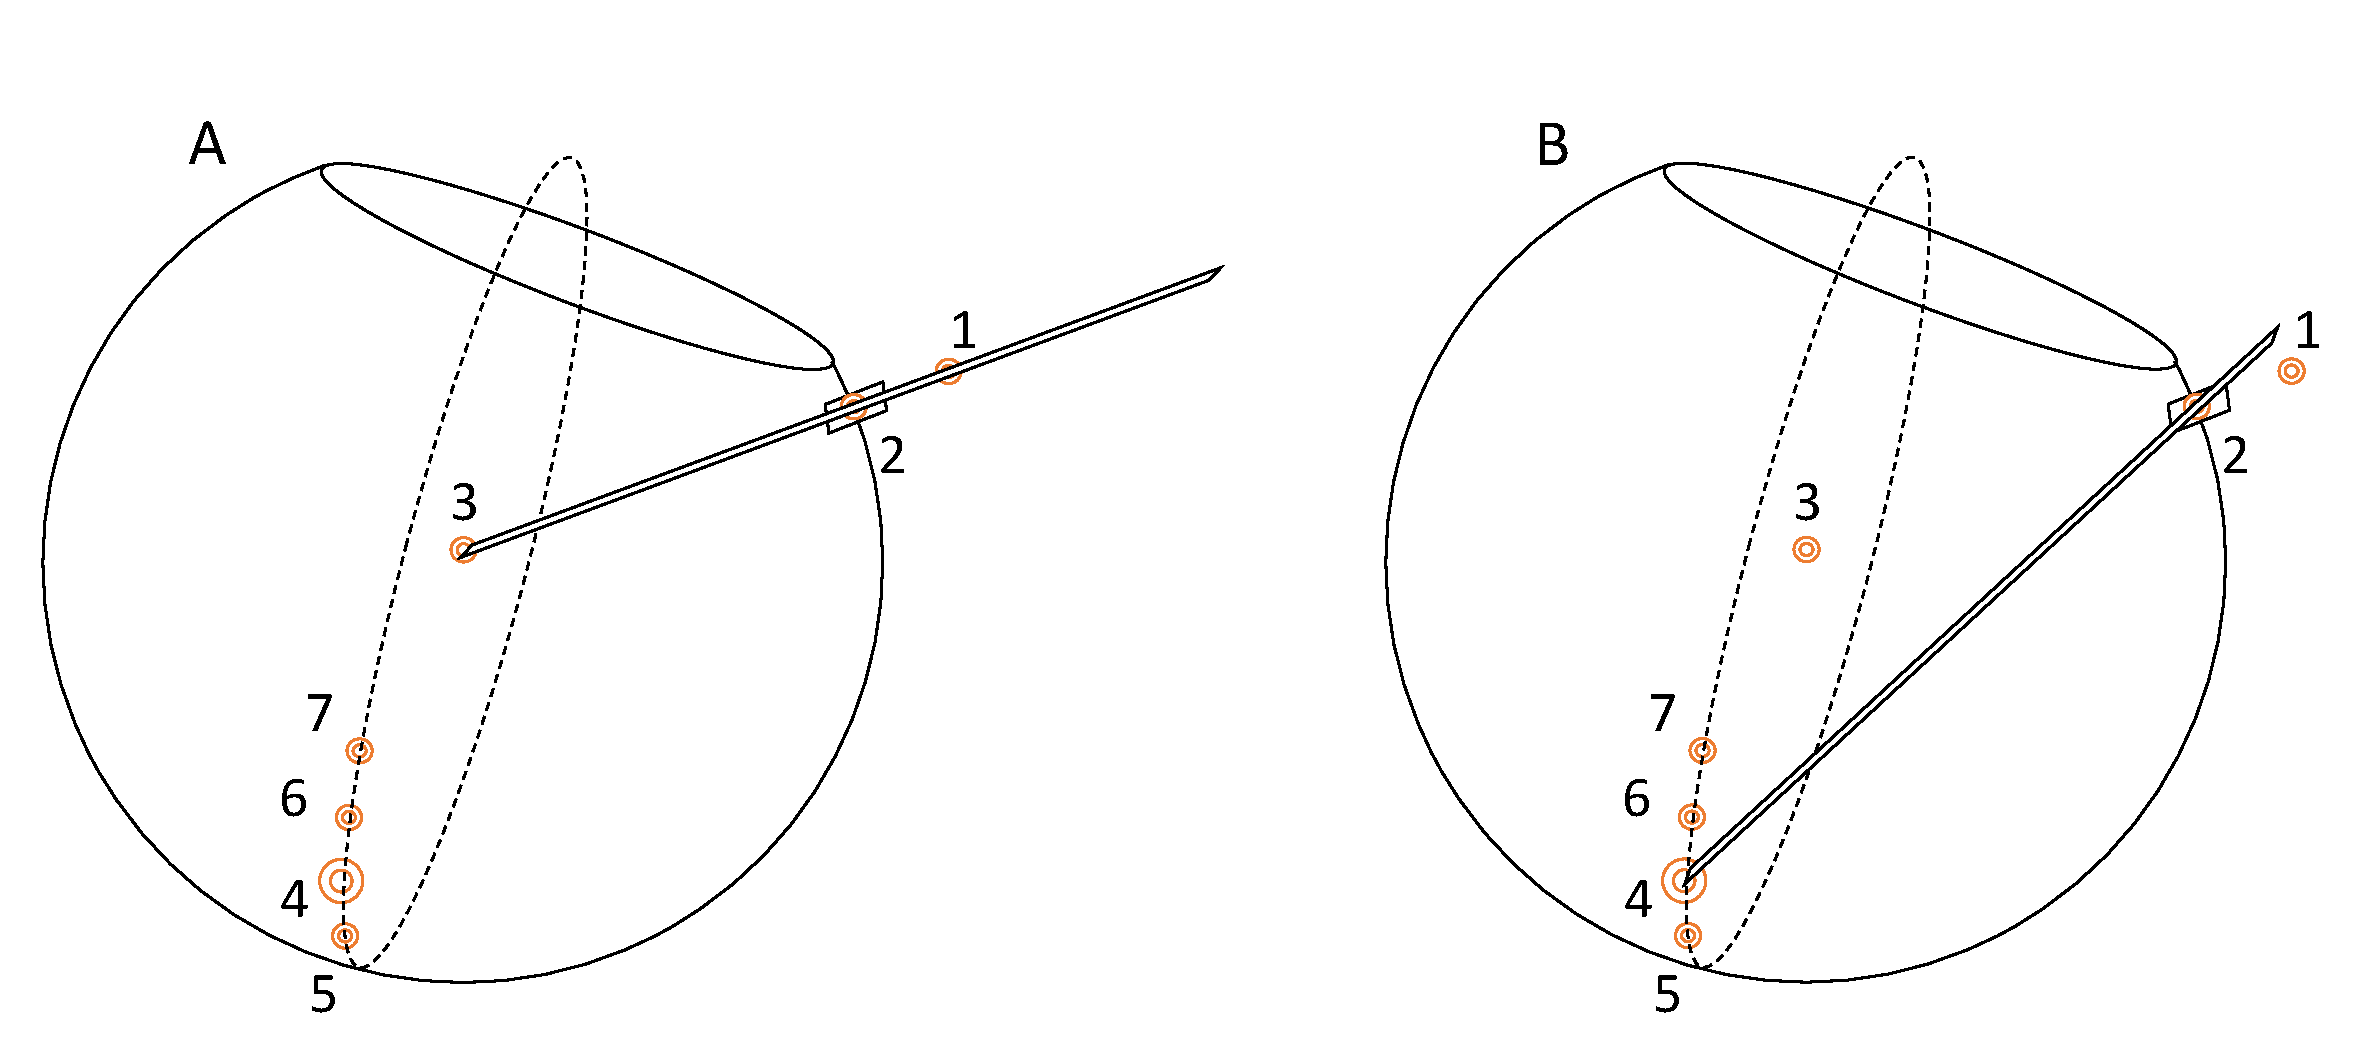
\includegraphics[width=400pt]{injection_illustration}
	\import{images/}{injection_illustration_refactored_tex.pdf_tex}\caption{Setup for measuring the precision of the RCM point. \textbf{A}: The needle enters the eye through the trocar until it reaches point \textbf{3}. \textbf{B}: The needle tip moves from point \textbf{3} to points \textbf{4}-\textbf{7} while keeping the RCM point, located at \textbf{2}, steady.}
	\label{injection_illustration}
\end{figure}

Injection begins by moving the tool tip from an arbitrary point outside the eye to position \textbf{2} via unconstrained movement. Once point \textbf{2} is reached, the RCM point will be positioned at the tip of the needle ($\lambda=1$) and control via the augmented Jacobian begins. The tool is pivoted around its tip until point \textbf{1} lies on the needle, and thus the needle is aligned with the trocar. The needle is then moved forwards in a straight line until its tip reaches point \textbf{3}. From there, points \textbf{4}-\textbf{7} located on the inner surface of the eye will be visited, returning to position \textbf{3} each time.

\section{Modelling the Surgical Robot in V-REP}

This section describes the process of generating two Simulation models that can be controlled via the MATLAB remote API from the CAD data of the robot: One model for use in forwards kinematics mode, where the slider positions $L_i$ are controlled via a MATLAB script according to the values computed by the Jacobian matrix, and one model for use in inverse kinematics mode, where only the target positions for the needle tip and the RCM are controlled by the MATLAB script and the joints are controlled by the internal IK solver.

The CAD model of the robot is first imported into V-REP as a single triangle mesh. Using the automatic mesh subdivision, a new shape is generated for all elements that are not connected via a common edge and thus, all components of the robot are extracted as separate rigid links. Now, joint objects are added to specify the movement of the links relative to each other. Figure \ref{vrep_model} shows the finished model of the robot.  

\begin{figure}[b!]
	\centering
	%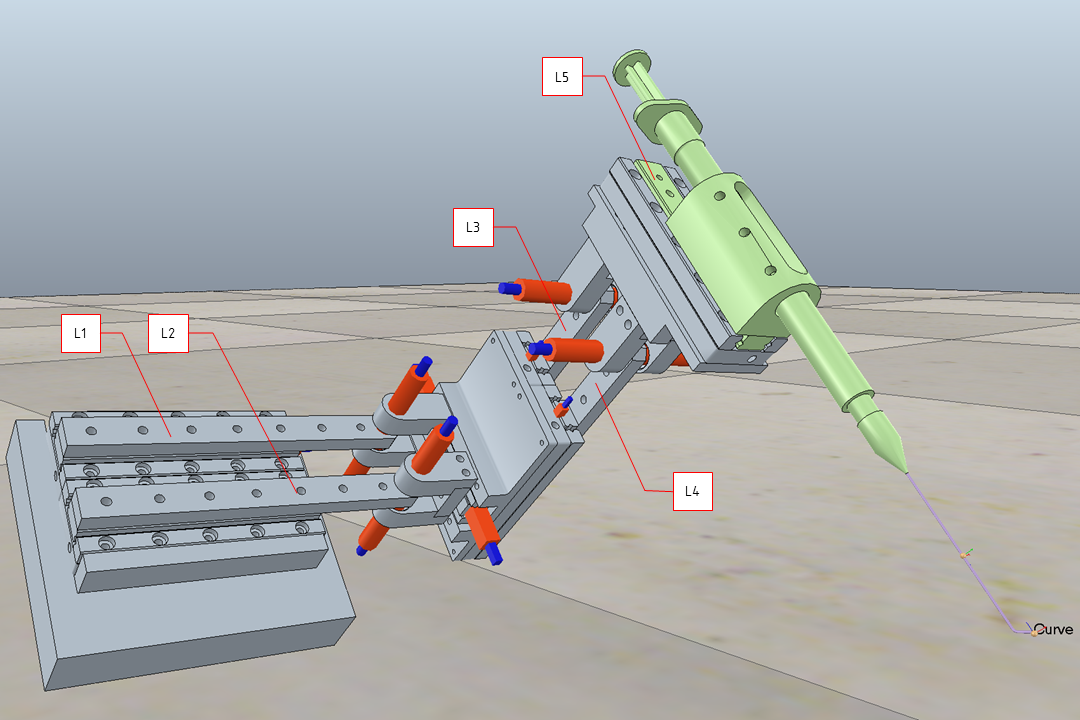
\includegraphics[width=300pt]{vrep_model}
	\import{images/}{vrep_model_1_tex.pdf_tex}
	\caption{The surgical robot modelled in V-Rep}
	\label{vrep_model}
\end{figure}

Next, we need to specify how the different links and joints are connected with each other. In the real robot, a PCJM consists of two sliders contribute that to the translation and rotation of a subsequent stage. This cannot be directly modelled in V-REP because each element (e.g. the middle stage) can only have one parent object (i.e. one of the sliders in the PCJM). To assemble the robot model into a single kinematic chain in which every object has only one parent element, we first connect the robot base plate with the needle via one slider of each PCJM (corresponding to $L_2$ and $L_4$). From the needle, we make our way back down towards the middle plate using slider $L_3$ and from the middle pate to the base plate via slider $L_1$. Since this second pair of sliders $L_3$ and $L_1$ is now "dangling" from their respective target plate (indicated by a green overlay in Figure \ref{vrep_hierarchy}) we need to inform the simulation that the two sliders should be connected to their respective base plates. Therefore, two sets of tip-target pairs are introduced. For each pair, one dummy is attached to the slider and one to the corresponding base plate and both are constrained to overlap in position and orientation (indicated by blue dotted arrows in Figure \ref{vrep_hierarchy}).     

\begin{figure}[t!]
	\centering
	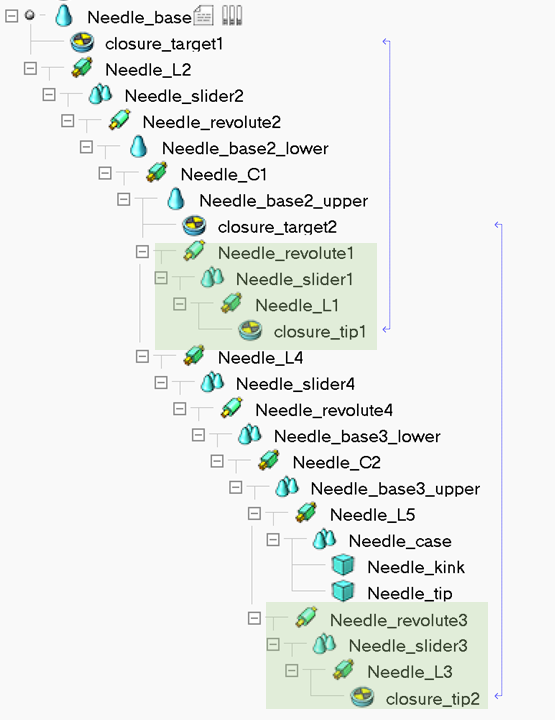
\includegraphics[width=8cm]{vrep_hierarchy}
	\caption{The scene hierarchy for the finished robot model. The green boxes indicate the sidearms of the kinematic chain that need to be constrained to be connected to their respective base plate via a tip-target pair (blue arrows).}
	\label{vrep_hierarchy}
\end{figure}

Until now, the modelling process has been the same for the forwards and inverse kinematics model. If we want to control the robot in forwards kinematics mode, the five prismatic joints corresponding to the stick-slip piezo actuators are set to "Force/Torque" mode and all other joints are set to "passive mode", meaning that they will not be actuated but can be passively rotated or displaced by connected moving links. For the inverse kinematics model, \textbf{all} joints are put into inverse kinematics mode so they can be controlled by the inverse kinematics solver. Additionally, we need to define the inverse kinematic task for the robot, described in the next section.

\subsection{Defining the Inverse Kinematic Task}

\begin{figure}[h!]
	\import{images/}{IK_refactored_2.pdf_tex}
	\caption{Schematic overview of the kinematic chain in V-REP. Objects connected by a bold black arrow indicate the primary kinematic chain which corresponds to the simplified serial robot in \ref{Manipulator}. Objects within a grey box belong to the same stage of the robot, i.e. one of the PCJMs or the final prismatic stage. A total of 4 IK pairs illustrated by yellow rings constrain (1) the position of the needle tip (2) the position of the RCM and (3,4) the position of the second slider within each PCJM}
	\label{IK_chain}
\end{figure}

Figure \ref{IK_chain} shows the kinematic chain used to define the inverse kinematics task. Since the robot consists of subsequent PCJMs, it cannot be modelled as a linear kinematic chain (every element can only have one parent in the scene hierarchy). Instead, three distinct IK groups that are defined. The first IK group governs the position of both the tool tip and the RCM point by finding a joint configuration that minimizes the distance to their respective targets. The tip and RCM position need to be included in the same IK group since they are on the same rigid link and in a way represent conflicting goals for the needle pose between which a compromise needs to be found. The other two IK groups are used to 'close the loop', that is to connect the side chains to their respective bottom plates. The two loop-closure IK tasks are added solely for cosmetic reasons, since even without them the position of the second slider in each PCJM could be uniquely reconstructed from the position of the first slider and the angle of the subsequent revolute joint.

\chapter{Results}

In this chapter the accuracy of the RCM point when performing injections at different sites on the inner surface of the eye will be evaluated using the method described in \ref{Setup}. Additionally, the choice of control parameters for the augmented Jacobian method will be discussed.

\section{Accuracy of the Jacobian Pseudoinverse Method} \label{Acc_PI}

\subsection{Choosing the Matrix K} \label{K}
When controlling the motion of the tool with the augmented Jacobian matrix, two parameters should be optimized: the control matrix \textbf{K} and the step size of the robot s which determines the magnitude of the change in joint positions for each iteration. Recalling Eqn. \ref{K_J}, we can see that each entry in \textbf{K} gives a weight to the error of one component in the pose, i.e. if one entry in \textbf{K} is large, the error in that component will converge to zero faster. On the other hand, two of the components in the pose vector are angles in radians, while the others are cartesian positions given in meters. The Jacobian matrix does not 'know' about these different length scales, thus the matrix \textbf{K} needs to correct for it. Additionally, the two angles have different levers with respect to the needle tip position, i.e. a change of 0.1 radians for both angles will result in a different displacement of the needle tip in y and z direction.  As a rough correction for this, we can calculate the approximate change in the position of the tip per angle of the robot is in its initial configuration ($q_i = 0$). 
For a small change of angle in $q_1$ and $q_3$, the change of the z- and y-position of the needle tip is given by 
\begin{align*}
\Delta z&=\sin\Delta q_1 \sqrt{l_2^2+l_6^2}\\
\Delta y&=\sin\Delta q_1 \sqrt{l_5^2+l_6^2}
\end{align*}
This gives us an approximate correction factor of 10 for the entries of \textbf{K} corresponding to the angular errors. Thus, we start optimization with \textbf{K}=diag([1, 10, 10, 1, 1, 1]). 

\subsection{Error in the RCM Position}

In Section \ref{control} a control loop was introduced which iterates until the robot's current pose matches a given target pose within a predefined magnitude. Large distances between start and target pose require a high number of iterations to converge because the Jacobian matrix attempts to correct the parameter with the largest error in one iteration, thereby displacing the other parameters heavily. These then return to their desired values in subsequent iterations as illustrated in Figure \ref{large_step}. This behaviour can be efficiently suppressed by splitting the full trajectory into several smaller parts. If the distance between these intermediate target positions is sufficiently small the control loop will converge from one position to the next within a small number of iterations without excessive overshooting.

\begin{algorithm}[t!]
 \begin{algorithmic}[1]
  \STATE $\textbf{start\_pose} \leftarrow \textit{get\_task\_pose}()$
  \STATE $\textbf{total\_distance} \leftarrow \textbf{target\_pose} - \textbf{start\_pose}$
  \STATE $\textbf{step} \leftarrow \textbf{total\_distance} / abs(\textbf{total\_distance}) \cdot \text{step\_size}$
  \WHILE {$max(abs(\textbf{target\_pose}-\textbf{current\_pose})) > 0.0003$}
   \STATE $\textbf{intermediate\_target\_position} \leftarrow \textbf{current\_pose} + \textbf{step}$
   \STATE $\text{Control\_Loop}(\bm{K}, \textbf{intermediate\_target\_position}, J_a, \lambda)$
   \STATE $\textbf{current\_pose} \leftarrow \textit{get\_task\_pose}()$
   \ENDWHILE 
 \end{algorithmic}
 \caption{$\text{Extended\_Control\_Loop}(\textbf{target\_pose}, \text{step\_size})$}
 \label{alg:ext_control_loop}
\end{algorithm}

\begin{figure}[b!]
	\begin{center}
		%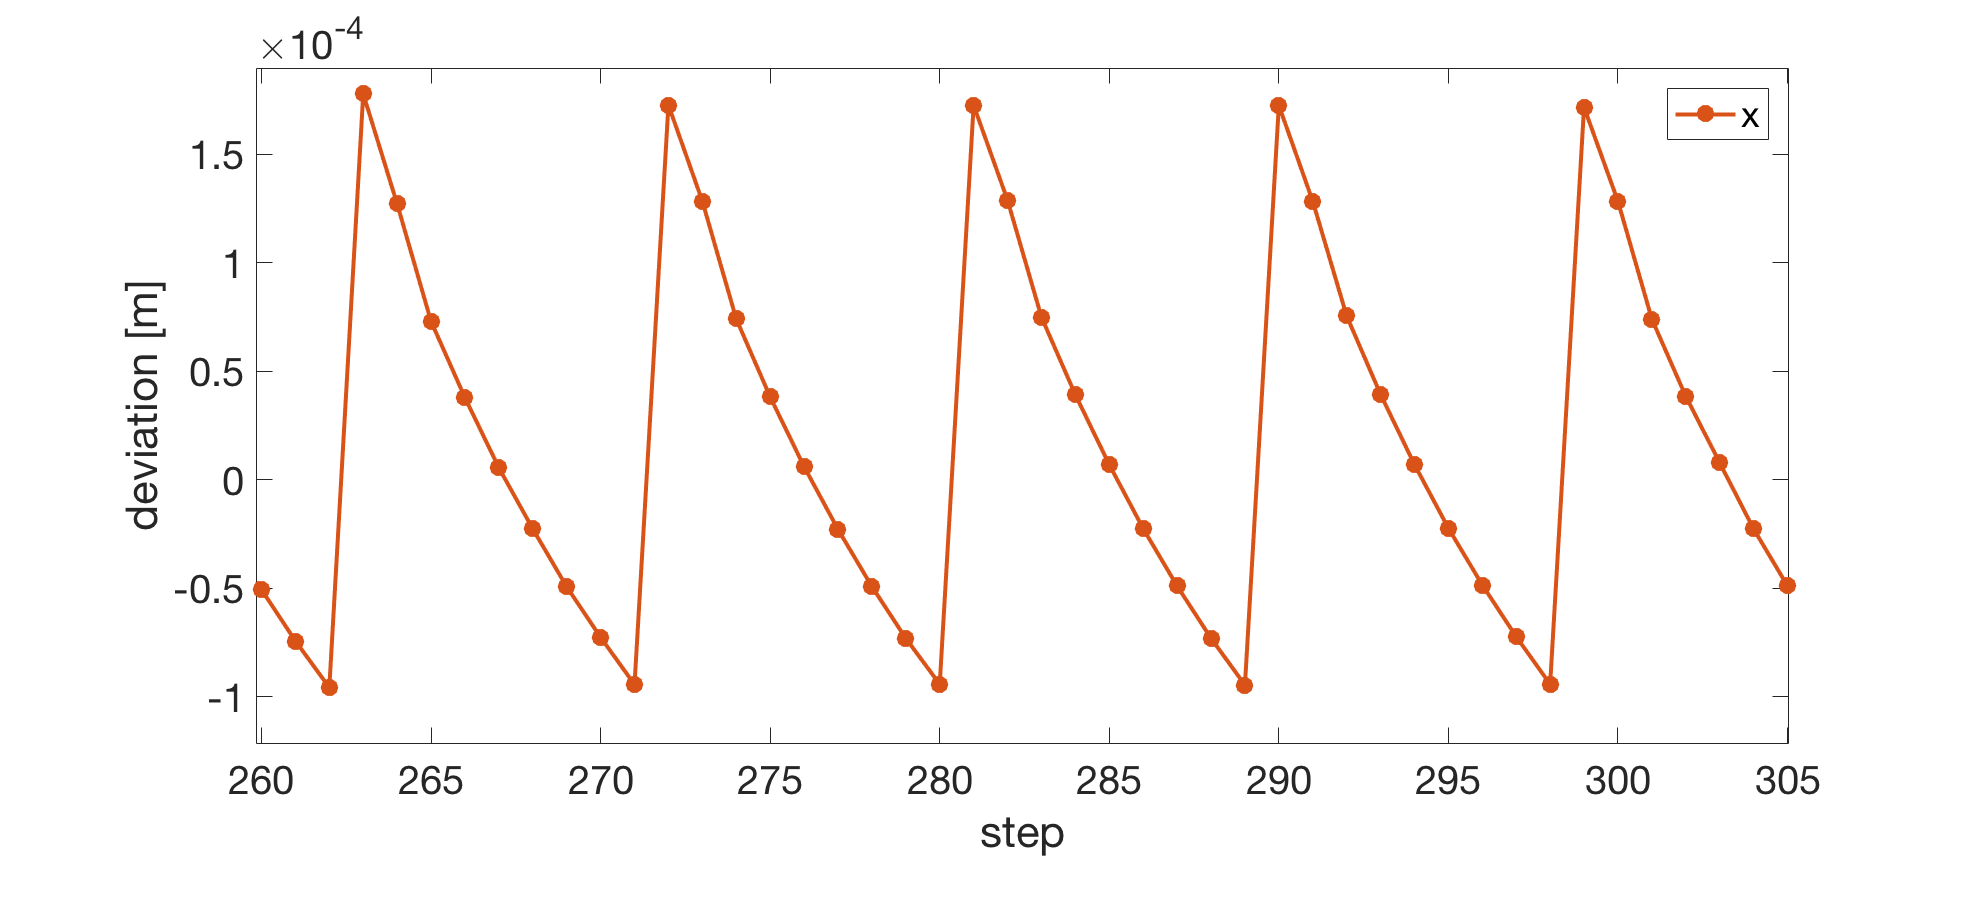
\includegraphics[width=15cm]{large_step}
		\import{images/}{large_step_tex.pdf_tex}
		\caption{Error in the RCM position when performing a step that is too large. The step starts with a large displacement in one direction and requires many iterations of the control loop to return to the desired RCM position.}
		\label{large_step}
	\end{center}
\end{figure}

The process of splitting the trajectory is illustrated in Algorithm \ref{alg:ext_control_loop}. given a target pose that is far away from the current pose, the extended control loop splits the trajectory in many small steps of equal length, determined by the step size. For each small step, the control loop presented in Section \ref{control} is executed, which brings the needle from the current position sufficiently close to the intermediate target. After the intermediate target is reached, a new small step in the direction of the target pose is calculated and again executed by the first control loop presented in Section \ref{control}.

\begin{figure}[b!]
	\begin{center}
		%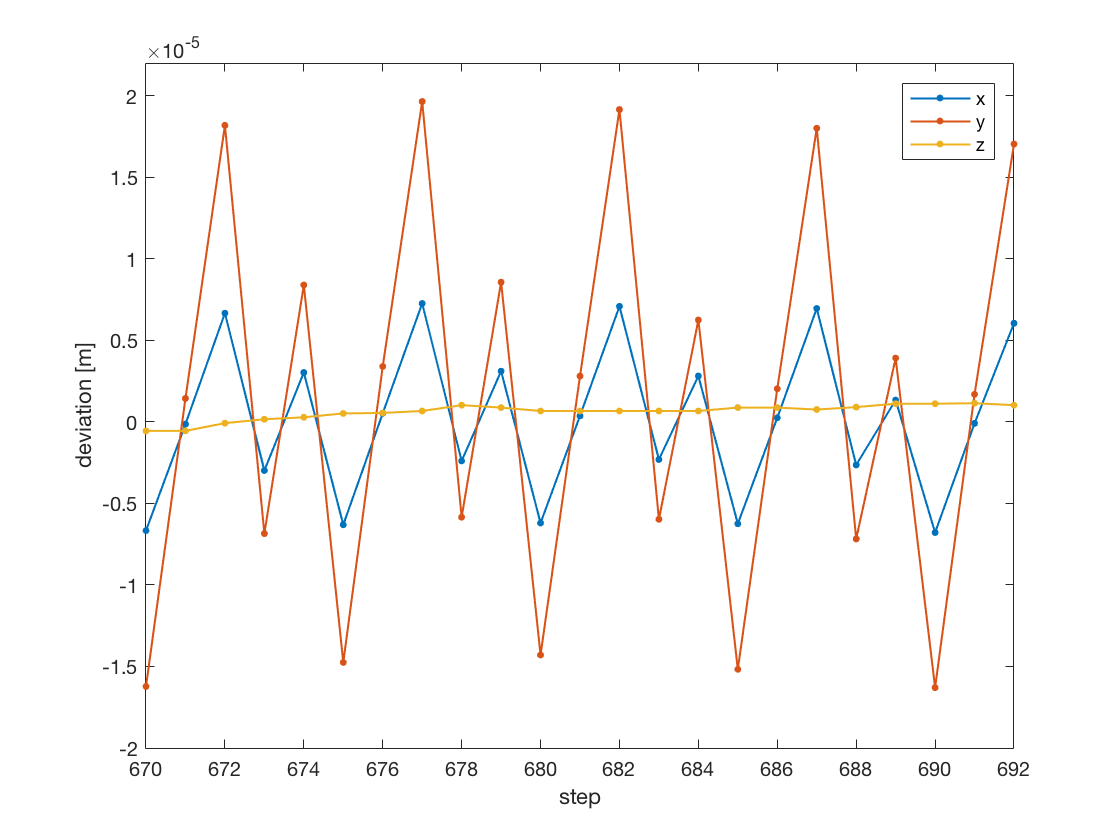
\includegraphics[width=15cm]{alignment_error_section_png}
		\import{images/}{alignment_error_section_refactored.pdf_tex}
		\caption{Error in the RCM position during 22 iterations of pivoting the needle around its tip during the alignment process described in Section \ref{Setup}.}
		\label{error_align_overall}
	\end{center}
\end{figure}

As an example for a proper choice in step size, two parts of the injection process are shown: The alignment of the needle with the trocar (at point 2 in Section \ref{Setup}), in which the RCM point is positioned at the needle tip ($\lambda=1$) and the entire robot pivots around its tip, as well as the movement from point 3 to point 7. These two were chosen because one illustrates the 'worst case' in terms of keeping the RCM point steady (as a small angle change leads to a large displacement of the RCM due to the long lever) and the other requires simultaneous adjustment of both angles of the needle while maintaining the RCM point.

Figure \ref{error_align_overall} shows the overall position of the RCM point during the alignment process. 500 steps according to the control loop in Section \ref{control} were performed to correct the angles $\Phi$ and $\Psi$ by $0.0048$ rad ($\approx 0.28$ deg) and $0.212$ rad ($\approx 12.12$ deg), respectively. In each of these steps, roughly 3 iterations were needed to ensure the accuracy of the RCM, resulting in a total of 1350 data points. The total computation time for this section of the injection process was about 3 minutes, which is quite a lot but was required to reach a high precision for the RCM point. During many iterations of this injection step, $K=diag([1 10 12 1 2 2])$ proved to be a good choice for the control matrix as a compromise between speed and accuracy.

\begin{figure}[b!]
	\begin{center}
		%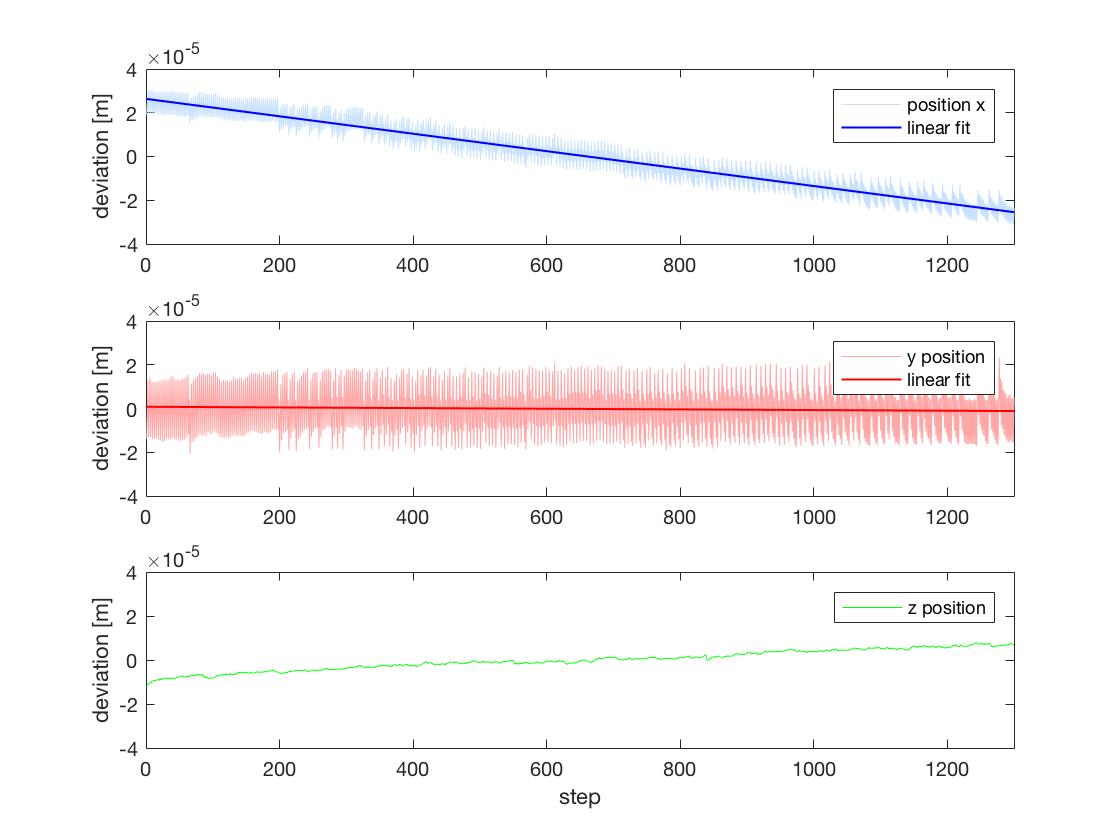
\includegraphics[width=15cm]{drift}
		\import{images/}{drift_tex.pdf_tex}
		\caption{ Overall error in the RCM position for the alignment of the needle with the trocar as proposed in Section \ref{Setup}. }
		\label{error_align}
	\end{center}
\end{figure}

The first thing to note about Figure \ref{error_align_overall} is that both $y_{rcm}$ and $z_{rcm}$ remain roughly constant during the entire procedure while $x_{rcm}$ experiences some drift. This drift occurs only in x-direction because the weight in $\bm{K}$ associated with $x_{rcm}$ is only half as large as the weights associated with $y_{rcm}$ and $z_{rcm}$.  When adjusting the values in $\bm{K}$, it is always necessary to find a good trade-off between accuracy of the RCM position and computation speed. By setting the weight related to $x_{rcm}$ to 2 instead of 1 the drift is reduced but the needle pose converges to the target pose much slower because the change in x-position competes with the change in both $\Psi$ and $\Phi$. In this example, the drift of $x_{rcm}$ during the alignment process is only $\pm3\cdot10^{-5}m$ which is negligible compared to the radius of the trocar which is about $45\cdot10^{-5}m$.

Both Figure \ref{error_align_overall} and \ref{error_align} illustrate the influence of the step size on the accuracy of the RCM point. A total of 500 steps are performed to align the needle with the trocar, but one of the initial angles is much closer to the target angle than the other. As a  result one angle will have a larger error each step and the Jacobian will calculate a larger $\Delta L$ to correct the angle, thus displacing the RCM more in one direction than the other. In this example the error in angle $\Psi$ is large, thus each step the needle will rotate about the z-axis by a large amount and as a result displace the RCM point in y direction. the error in angle $\Phi$ is very small and thus the RCM is hardly displaced in z-position. The x-position, which roughly corresponds to the depth the needle is injected into the eye, is affected by both angle changes, therefore its error is somewhere in between.

Figures \ref{3_7} and \ref{3_7_drift} show the error per step and the overall drift and  for the RCM point during the movement from point $3$ to point $7$ proposed in Section \ref{Setup}. Both are very similar in precision to the ones for the alignment with the trocar which shows that simultaneous adjustment of two angles does not significantly decrease performance. The total computation time for this section of the injection was roughly 2 minutes. 

 \begin{figure}[t!]
	\begin{center}
		%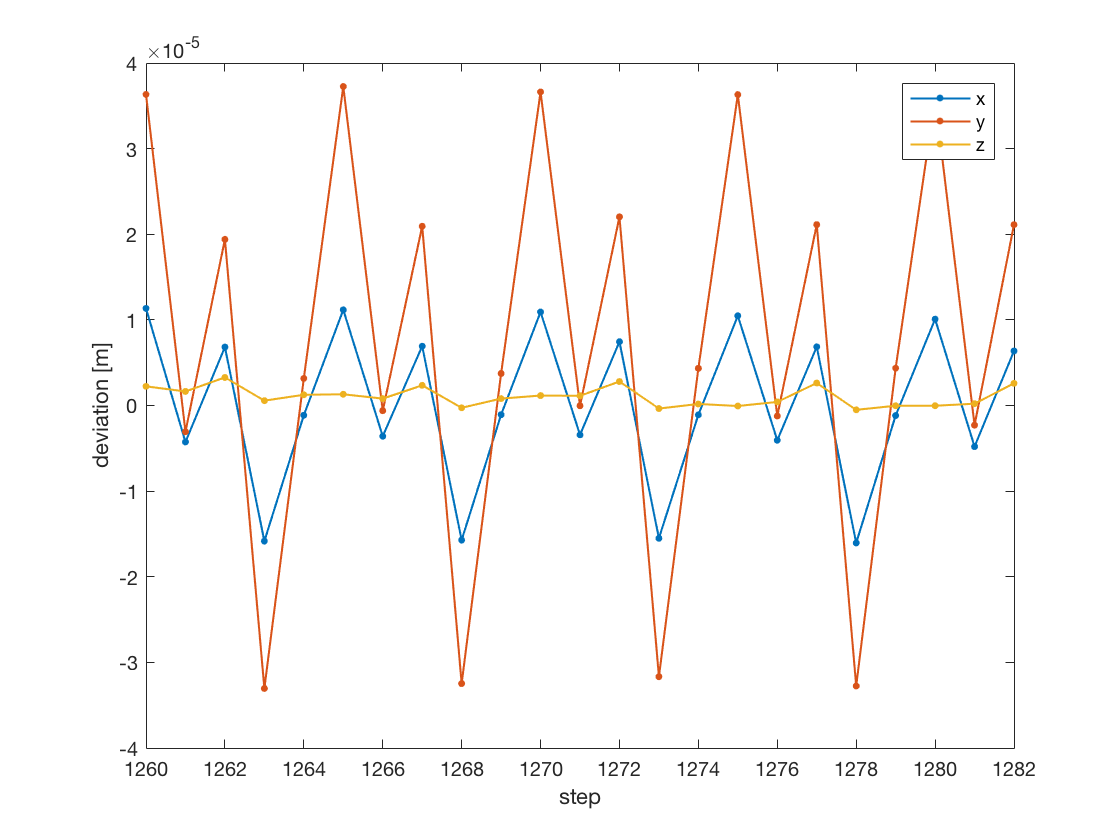
\includegraphics[width=15cm]{3_7}
		\import{images/}{3_7_tex.pdf_tex}
		\caption{ Error in the RCM position during 22 iterations of the movement  from point $3$ to point $7$ as proposed in Section \ref{Setup}.}
		\label{3_7}
	\end{center}
\end{figure}

\begin{figure}[t!]
	\begin{center}
		%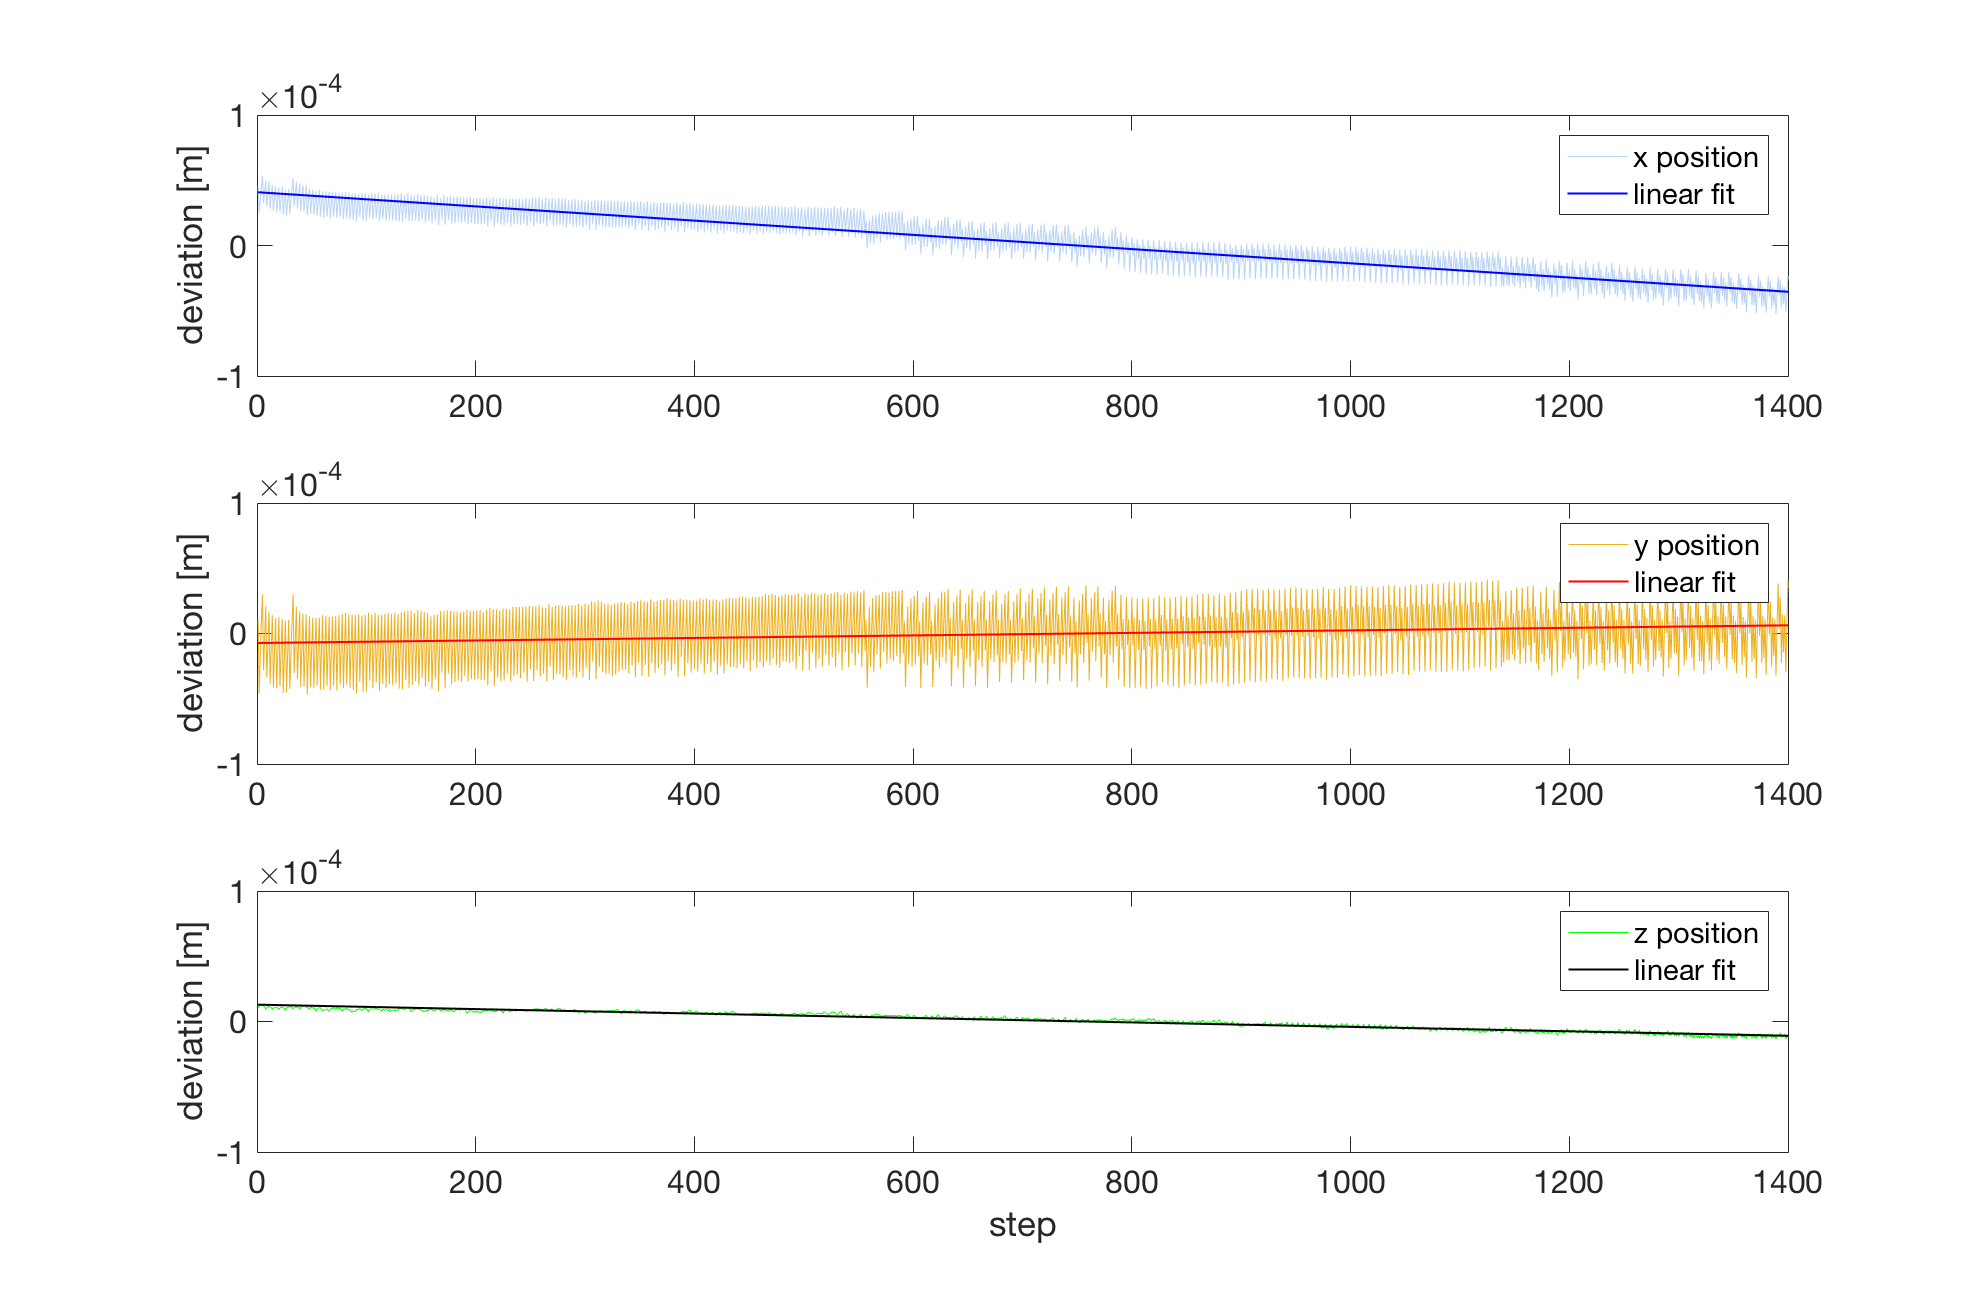
\includegraphics[width=15cm]{3_7_drift}
		\import{images/}{3_7_drift_tex.pdf_tex}
		\caption{ Overall error in the RCM position for the movement from point $3$ to point $7$ as proposed in Section \ref{Setup}. }
		\label{3_7_drift}
	\end{center}
\end{figure}

\section{Accuracy of the Dampened Least Squares Method} \label{Acc_DLS}

This section discusses the accuracy of V-REPs inverse kinematic solver which utilizes the Levenberg-Marquardt algorithm discussed in Section \ref{DLS}. The DLS algorithm functions very similarly to the Jacobian pseudoinverse method in that it linearises the IK problem near the current pose via the Jacobian matrix. There are two key points in which the DLS algorithm improves upon the Jacobian pseudoinverse approach: Firstly, the DLS algorithm introduces the damping parameter $D$ which prevents the algorithm from running into numeric instability close to a singularity. Secondly, the DLS algorithm never performs a matrix inversion, improving its computation time especially for Manipulators with a large number of links.
For the robot considered in this thesis, the DLS algorithm should not have a significantly higher performance than the pseudoinverse method, given an optimal choice for the matrix $\bm{K}$ and a sufficiently small step size, because there are no singularities in the workspace of the robot. Thus, to give an idea about the precision that is possible to achieve with the augmented Jacobian method the precision of the built-in IK solver is evaluated. Figure \ref{DLS_method} shows the setup used for showcasing the precision of the Dampened Least Squares Method. An off-axis spiral is drawn with the needle tip, keeping the RCM point steady at all times. Figure \ref{DLS_result} shows the deviation of the RCM point. The damping factor $D$ is set to 0.1.  

\begin{figure}[h!]
	\begin{center}
		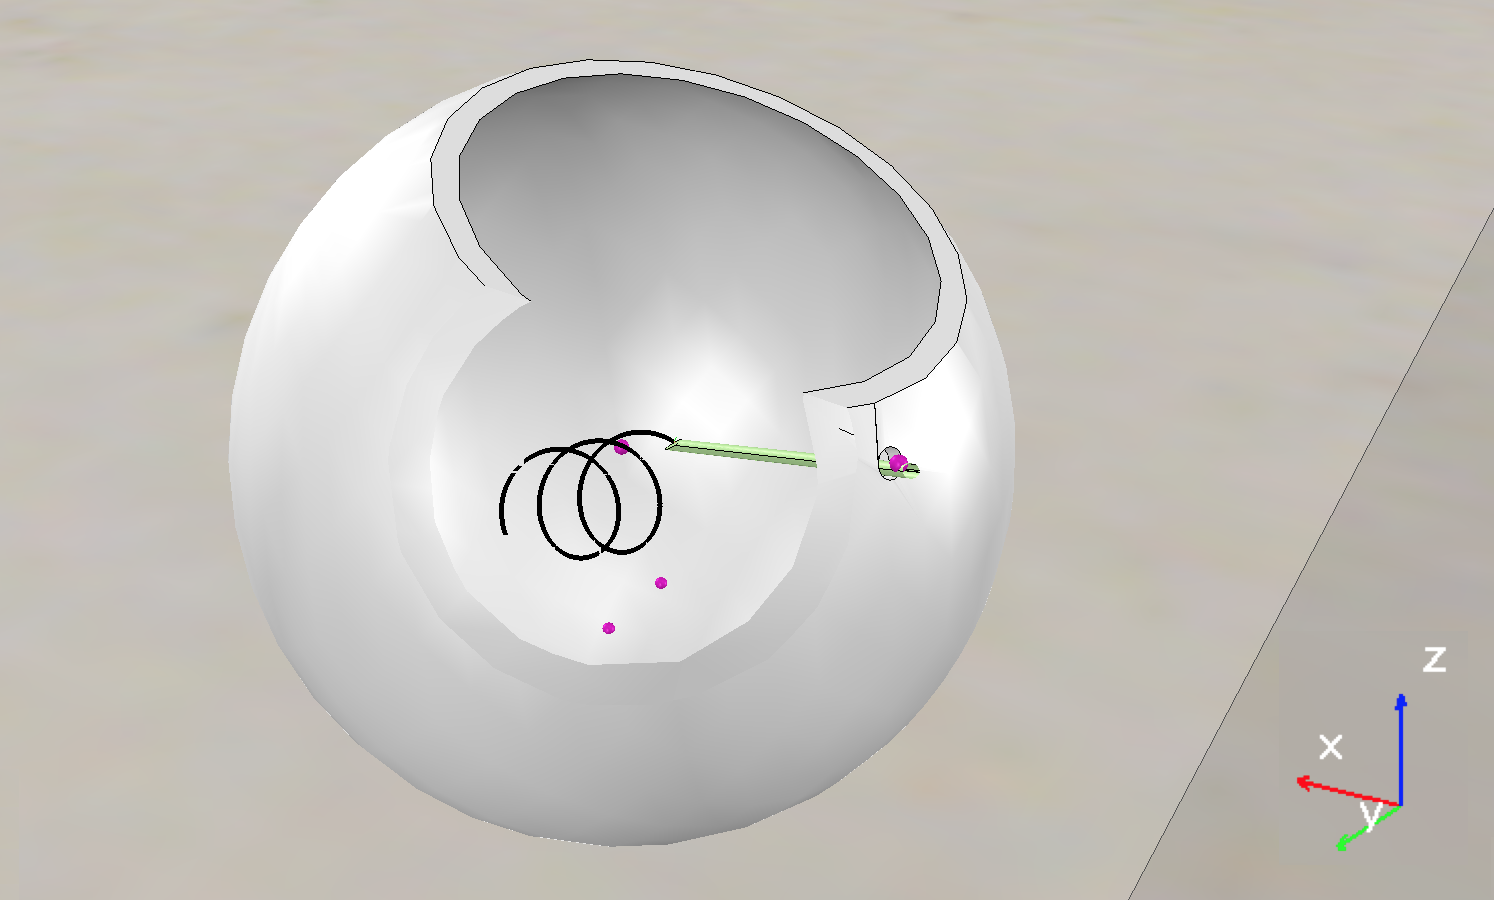
\includegraphics[width=15cm]{vrep-benchmark}
		\caption{Needle tip of the Robot tracing the shape of a spiral within the eye while keeping the RCM point steady, using V-REPs inverse kinematics module. The trajectory was recorded by V-REP using a graph object positioned at the needle tip. }
		\label{DLS_method}
	\end{center}
\end{figure}

\begin{figure}[h!]
	\begin{center}
		%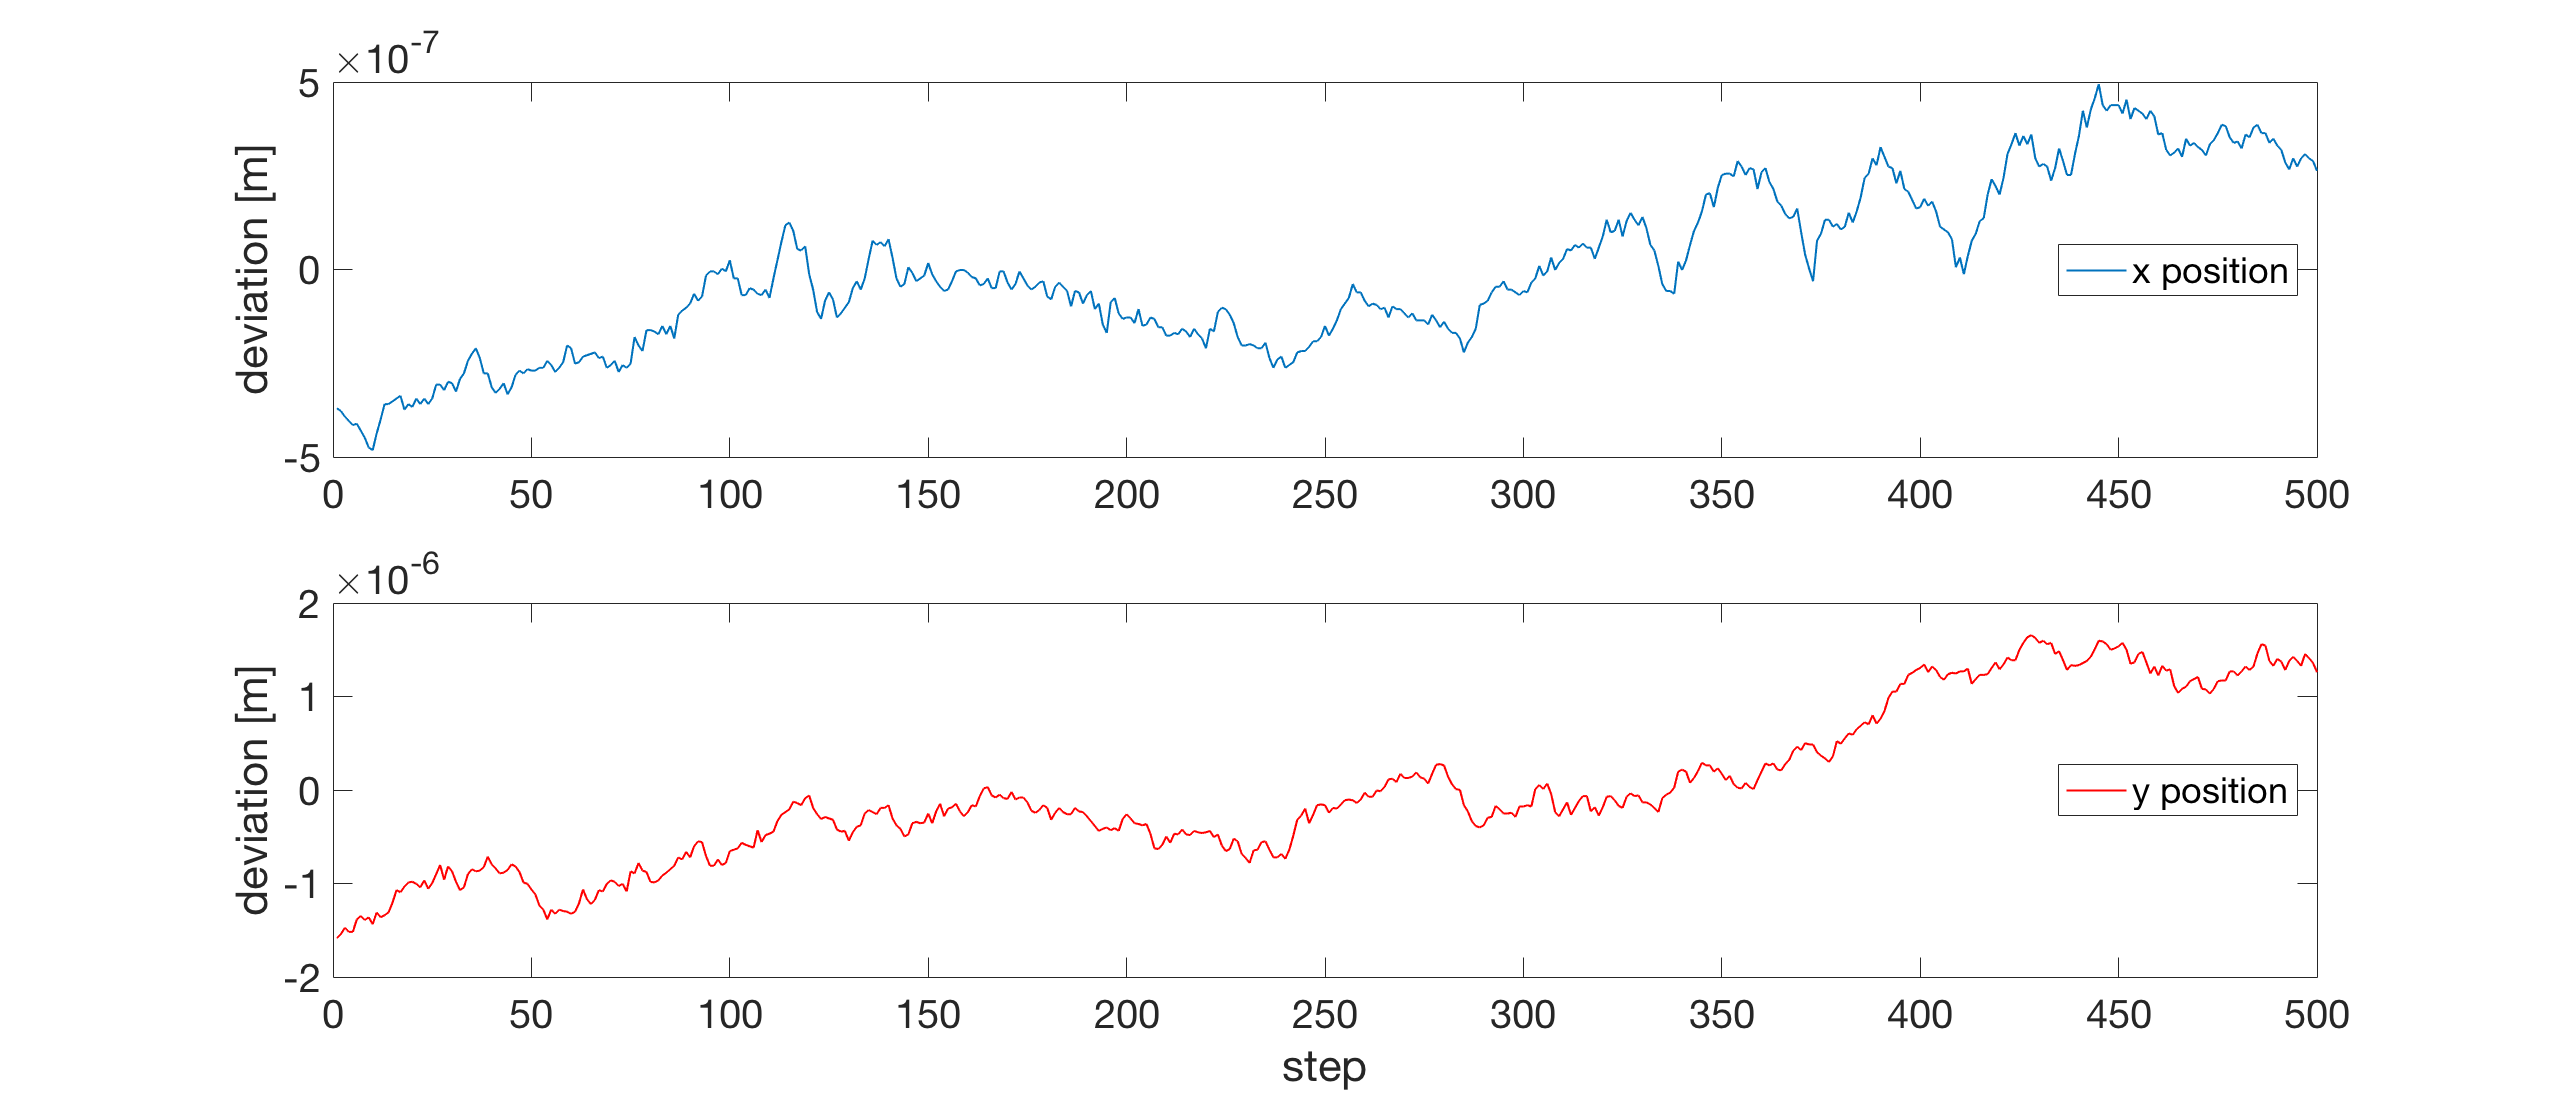
\includegraphics[width=16cm]{IK_solution}
		\import{images/}{IK_solution_tex.pdf_tex}
		\caption{Error in the RCM position during the first 500 calculation steps of the V-REP IK solver, producing the trajectory seen in Figure \ref{DLS_method}.}
		\label{DLS_result}
	\end{center}
\end{figure}

The accuracy of the DLS method proved to be extremely high compared to the Jacobian pseudoinverse method. Furthermore, the computation time to draw the shape in Figure \ref{DLS_method} was only 28 seconds. although the minimum precision was set to 0.1mm, the method seemed to be much more precise, implying that a smaller damping factor could have been chosen to speed up computation even more. 

\chapter{Conclusion}

The results in the previous section show that control of the robot via the augmented Jacobian matrix is a valid approach to solving the inverse kinematics problem. When performing sufficiently small steps the deviation of the RCM from its ideal position was small enough as to not put stress on the tissue surrounding the incision site. Even though the method proved to be precise enough in simulation, the precision for the real robot would most likely be lower since no dynamic effects were considered. To improve the overall accuracy, there are several points that can be relatively easily implemented building on the results presented but exceed the scope of this thesis. These include: 

\paragraph{Preventing drift of the RCM position:} As discussed in Section \ref{Acc_PI}, the x-position of the RCM point experiences some drift during the course of the injection. While the drift is relatively small compared to the size of the trocar, a proper solution might significantly increase the performance. Within each iteration step, the RCM is forced to the target position ($x_{rcm}, y_{rcm}, z_{rcm}$), allowing a small deviation from the target position as a trade-off between drift rate and computation time. By adjusting the corresponding entry in the matrix $K$, the error of $x_{rcm}$ is given a higher priority and will drift less, but all other position parameters will converge slower leading to a worse overall performance. This problem might be easily resolved by readjusting the position of the RCM on the needle in each iteration step before enforcing the normal control loop. This means that before each iteration the point on the needle closest to ($x_{rcm}, y_{rcm}, z_{rcm}$) is calculated and declared as the new RCM point. 

\paragraph{Improving the control matrix $\bm{K}$:} The control matrix $K$ used in this thesis was determined empirically and proved to be a good trade-off between accuracy and convergence speed. However, it is certainly not optimal for every kind of movement within the workspace of the robot inside the eye, as it was adjusted using only the injection procedure presented in Section \ref{Setup}. A better $K$ can be determined by systematically computing accuracy and convergence during movements within the whole workspace inside the eye for different combinations of entries in $K$.

\paragraph{Inclusion of a third rotation into the Jacobian matrix and simulation:} The model of the surgical robot considered in this thesis uses a straight needle as a tool, thus the rotation around the tool axis has no effect on the position of the needle tip and can be neglected. Having established the kinematic relationships in the robot model and a strategy to calculate both the unconstrained and augmented Jacobian matrix, a needle with a curved tip can be implemented. A curved needle allows for injections lateral to the surface and extends the reachable surface area for injection inside the eye, but makes it more difficult to enter the eye through the trocar while maintaining the RCM point. To implement this, the Jacobian matrix needs to be extended by one row expressing the rotation of the tool around its own axis and the augmented Jacobian matrix must be updated accordingly.

\paragraph{Inclusion of dynamic effects into the Simulation:} The V-REP simulation environment is capable of performing precise dynamic calculations. It might be interesting to estimate the loss in precision of both inverse kinematics methods when dynamic effects are considered. 
\chapter{Appendix}

\hspace{3cm}
\rotatebox{90}{
  \begin{minipage}{18cm}
	\begin{eqnarray}
	J_a =
		\begin{bmatrix}
			0	& l_2 c1 + l_6 c3 s1 + l_5 s1 s3 + q_4 c3 s1			& 0& c1 (l_6 s3 - l_5 c3 + q_4 s3)				& -c1 c3	& 0			\\
			0	& 1											& 0& 0									& 0		& 0			\\
			0	& 0											& 0& c1									& 0		& 0			\\
			0	& l_2 c1 + l_5 s1 s3 + q_4 c3 s1 + l_6 \lambda c3 s1	& 0& c1 (q_4 s3 - l_5 c3 + l_6 \lambda s3)		& -c1 c3	& -l_6 c1 c3	\\
			0	& 0											& 1& - l_5 s3 - q_4 c3 - l_6 \lambda c3			& -s3	& -l_6 s3		\\
			1	& l_5 c1 s3 - l_2 s1 + q_4 c1 c3 + l_6 \lambda c1 c3	& 0& -s1 (q_4 s3 - l_5 c3 + l_6 \lambda s3)		& c3 s1	& l_6 c3 s1	\\
		\end{bmatrix}\label{J_a_full}
	\end{eqnarray}
	\hspace{1cm} with $ci,si := \cos(i), \sin(i)$.
  \end{minipage}
}

% Matlab output:
%J_ext=	[
%	0, L2*cos(q1) + L6*cos(q3)*sin(q1) + L5*sin(q1)*sin(q3) + q4*cos(q3)*sin(q1), 0,         cos(q1)*(L6*sin(q3) - L5*cos(q3) + q4*sin(q3)), -cos(q1)*cos(q3),                   0;
%	0,                                                                                1, 0,                                                      0,                0,                   0;
%	0,                                                                                0, 0,                                                cos(q1),                0,                   0;
%	0, L2*cos(q1) + L5*sin(q1)*sin(q3) + q4*cos(q3)*sin(q1) + L6*lambda*cos(q3)*sin(q1), 0,  cos(q1)*(q4*sin(q3) - L5*cos(q3) + L6*lambda*sin(q3)), -cos(q1)*cos(q3), -L6*cos(q1)*cos(q3);
%	0,                                                                                0, 1,          - L5*sin(q3) - q4*cos(q3) - L6*lambda*cos(q3),         -sin(q3),         -L6*sin(q3);
%	1, L5*cos(q1)*sin(q3) - L2*sin(q1) + q4*cos(q1)*cos(q3) + L6*lambda*cos(q1)*cos(q3), 0, -sin(q1)*(q4*sin(q3) - L5*cos(q3) + L6*lambda*sin(q3)),  cos(q3)*sin(q1),  L6*cos(q3)*sin(q1)
%		];


% after replacement:
%J_ext=	[ 
%	0& l_2 c1 + l_6 c3 s1 + l_5 s1 s3 + q4 c3 s1& 0&         c1 (l_6 s3 - l_5 c3 + q4 s3)& -c1 c3&                   0\\
%	0&                                                                                1& 0&                                                      0&                0&                   0\\
%	0&                                                                                0& 0&                                                c1&                0&                   0\\
%	0& l_2 c1 + l_5 s1 s3 + q4 c3 s1 + l_6 lambda c3 s1& 0&  c1 (q4 s3 - l_5 c3 + l_6 lambda s3)& -c1 c3& -l_6 c1 c3\\
%	0&                                                                                0& 1&          - l_5 s3 - q4 c3 - l_6 lambda c3&         -s3&         -l_6 s3\\
%	1& l_5 c1 s3 - l_2 s1 + q4 c1 c3 + l_6 lambda c1 c3& 0& -s1 (q4 s3 - l_5 c3 + l_6 lambda s3)&  c3 s1&  l_6 c3 s1\\
%		]



%J_ext=	[ 
%	0& l_2*c1 + l_6*c3*s1 + l_5*s1*s3 + q4*c3*s1& 0&         c1*(l_6*s3 - l_5*c3 + q4*s3)& -c1*c3&                   0\\
%	0&                                                                                1& 0&                                                      0&                0&                   0\\
%	0&                                                                                0& 0&                                                c1&                0&                   0\\
%	0& l_2*c1 + l_5*s1*s3 + q4*c3*s1 + l_6*lambda*c3*s1& 0&  c1*(q4*s3 - l_5*c3 + l_6*lambda*s3)& -c1*c3& -l_6*c1*c3\\
%	0&                                                                                0& 1&          - l_5*s3 - q4*c3 - l_6*lambda*c3&         -s3&         -l_6*s3\\
%	1& l_5*c1*s3 - l_2*s1 + q4*c1*c3 + l_6*lambda*c1*c3& 0& -s1*(q4*s3 - l_5*c3 + l_6*lambda*s3)&  c3*s1&  l_6*c3*s1\\
%		]

\bibliographystyle{plain}
\bibliography{References}

\end{document}